% Compilação recomendada no Overleaf: pdfLaTeX
% Enviar a pasta parte2 inteira (figuras/, tabelas/ e codigo/ são lidas pelo documento)
\documentclass[12pt,a4paper]{article}

\usepackage[T1]{fontenc}
\usepackage[utf8]{inputenc}
\usepackage[brazilian]{babel}
\usepackage{lmodern}
\usepackage{microtype}
\usepackage[a4paper,margin=2.35cm]{geometry}
\usepackage{graphicx}
\usepackage{booktabs}
\usepackage{array}
\usepackage{float}
\usepackage{placeins}
\usepackage{enumitem}
\usepackage{amsmath,amssymb}
\usepackage{xcolor}
\usepackage{textcomp}
\usepackage{listings}
\usepackage{hyperref}
\usepackage{fancyhdr}

\hypersetup{
  colorlinks=true,
  allcolors=black,
  pdfborder={0 0 0},
  pdftitle={Atividade 2 -- Regressão Linear Múltipla},
  pdfauthor={Nicholas Kim; Luiz Eduardo da Silva; Paulo Henrique Froelich Gomes}
}

\setlength{\parindent}{1.1cm}
\setlength{\parskip}{0.35em}
\setlength{\headheight}{15pt}
\clubpenalty=10000
\widowpenalty=10000
\displaywidowpenalty=10000
\renewcommand{\arraystretch}{1.16}
\setlist[itemize]{leftmargin=1.35em,noitemsep,topsep=0.3em}
\pagestyle{fancy}
\fancyhf{}
\lhead{\footnotesize ACH2036 -- Métodos Quantitativos}
\rhead{\footnotesize Atividade 2}
\cfoot{\thepage}
\renewcommand{\headrulewidth}{0pt}

\newcommand{\Rtwo}{\ensuremath{R^2}}
\newcommand{\Rtwoadj}{\ensuremath{R^2_{\text{aj}}}}
\newcommand{\NA}{\textemdash}
\newcommand{\pval}[1]{\ensuremath{#1}}

% Blocos de código (scripts Python executados na análise)
\renewcommand{\lstlistingname}{Bloco}
\lstset{
  language=Python,
  basicstyle=\ttfamily\footnotesize,
  keywordstyle=\bfseries,
  commentstyle=\itshape\color{black!60},
  stringstyle=\color{black!80},
  showstringspaces=false,
  breaklines=true,
  columns=fullflexible,
  keepspaces=true,
  frame=single,
  rulecolor=\color{black!25},
  backgroundcolor=\color{black!3},
  framesep=4pt,
  xleftmargin=4pt,
  xrightmargin=4pt,
  aboveskip=0.9em,
  belowskip=0.7em,
  captionpos=t,
  upquote=true,
  extendedchars=true,
  inputencoding=utf8,
  literate=
    {á}{{\'a}}1 {à}{{\`a}}1 {â}{{\^a}}1 {ã}{{\~a}}1
    {é}{{\'e}}1 {ê}{{\^e}}1 {í}{{\'i}}1 {ó}{{\'o}}1
    {ô}{{\^o}}1 {õ}{{\~o}}1 {ú}{{\'u}}1 {ç}{{\c{c}}}1
    {Á}{{\'A}}1 {É}{{\'E}}1 {Í}{{\'I}}1 {Ó}{{\'O}}1
    {Ú}{{\'U}}1 {Ã}{{\~A}}1 {Ç}{{\c{C}}}1 {²}{{\textsuperscript{2}}}1
}

\begin{document}

\hypersetup{pageanchor=false}
\begin{titlepage}
  \raggedright
  \vspace*{1cm}
  {\large Universidade de São Paulo\par}
  \vspace{0.25cm}
  {\normalsize ACH2036 -- Métodos Quantitativos para Análise Multivariada\par}
  \vspace{3cm}
  {\Large Atividade 2\par}
  \vspace{0.5cm}
  {\huge\bfseries Regressão Linear Múltipla\par}
  \vspace{0.4cm}
  {\Large Valor do aluguel residencial em cinco cidades brasileiras\par}
  \vspace{2.5cm}
  {\normalsize
    \textbf{Nicholas Kim}\\
    Número USP 16990054\par
    \vspace{0.5cm}
    \textbf{Luiz Eduardo da Silva}\\
    Número USP 17018992\par
    \vspace{0.5cm}
    \textbf{Paulo Henrique Froelich Gomes}\\
    Número USP 15483136\par
  }
  \vfill
  {\normalsize São Paulo, 2026\par}
\end{titlepage}

\hypersetup{pageanchor=true}
\pagenumbering{roman}
\tableofcontents
\newpage
\pagenumbering{arabic}

% =====================================================================
\section{Problema de regressão a ser tratado}

A base utilizada é a \textit{Brazilian Houses to Rent}, publicada no Kaggle \cite{kaggle} e redistribuída no repositório OpenML com o nome \texttt{Brazilian\_houses} (ID 42688, versão 4) \cite{openml}. A versão do OpenML corresponde ao arquivo \texttt{houses\_to\_rent\_v2.csv} da base original e contém 10.692 anúncios de imóveis residenciais para locação em São Paulo, Rio de Janeiro, Belo Horizonte, Porto Alegre e Campinas, coletados por um \textit{web crawler} em sites de anúncios. Cada registro descreve o imóvel (cidade, área, quartos, banheiros, vagas de garagem, andar, aceitação de animais e mobília) e seus custos mensais: aluguel, condomínio, IPTU, seguro contra incêndio e o total desses valores. A única alteração do OpenML em relação ao arquivo original, segundo sua documentação, foi a substituição do andar ``-'' por 0; de acordo com o autor da base, esse código identifica casas.

O objetivo é avaliar a associação entre o valor mensal do aluguel (em R\$) e as características do imóvel, quantificando, por exemplo, quanto o aluguel varia entre as cidades, com a área, com o número de banheiros ou com a presença de mobília, mantidas constantes as demais características. Secundariamente, verifica-se se o modelo permite prever o aluguel de um novo anúncio com acurácia razoável.

A escolha foi motivada pela relevância do tema, pois o custo de moradia é uma preocupação direta de estudantes e trabalhadores nas grandes cidades, e pelas características da base, que exercitam as etapas de pré-processamento descritas no enunciado: resposta e preditoras fortemente assimétricas, variáveis categóricas, contagens, valores nulos legítimos, registros duplicados, valores implausíveis e duas variáveis que, se mantidas, transfeririam a própria resposta para o modelo.

Todo o processamento foi feito em Python, com as bibliotecas pandas, SciPy, statsmodels \cite{statsmodels} e Matplotlib. Conforme o enunciado, os scripts são apresentados em blocos ao longo do texto, cada um seguido de seus resultados parciais e da discussão correspondente. Os blocos são executados em sequência e compartilham as variáveis, como as células de um notebook; o script que os executa e as funções auxiliares de visualização estão no Apêndice~\ref{ap:auxiliar}. As tabelas foram exportadas diretamente dos resultados, e os valores foram arredondados somente para apresentação.

% =====================================================================
\section{Descrição da base}

\subsection{Dicionário de variáveis}

A Tabela~\ref{tab:dicionario} apresenta as variáveis da base. Os nomes originais foram substituídos por abreviações em português, utilizadas nos gráficos, nas tabelas e no código. A base não possui campos identificadores, como código do anúncio, endereço ou nome do anunciante; portanto, nenhuma coluna precisou ser suprimida por esse motivo.

\begin{table}[H]
\centering
\caption{Dicionário das variáveis.}
\label{tab:dicionario}
\footnotesize
\begin{tabular}{>{\raggedright\arraybackslash}p{1.85cm}
                >{\raggedright\arraybackslash}p{3.75cm}
                >{\raggedright\arraybackslash}p{4.35cm}
                >{\raggedright\arraybackslash}p{2.3cm}
                >{\raggedright\arraybackslash}p{1.6cm}}
\toprule
Abreviação & Nome original & Descrição & Tipo & Uso \\
\midrule
aluguel & \texttt{rent\_amount\_(BRL)} & Valor mensal do aluguel (R\$) & Contínua & Resposta \\
cidade & \texttt{city} & Cidade do imóvel: São Paulo, Rio de Janeiro, Belo Horizonte, Porto Alegre ou Campinas & Categórica não ordinal & Preditora \\
area & \texttt{area} & Área do imóvel (m$^2$), registrada em valores inteiros & Contínua & Preditora \\
quartos & \texttt{rooms} & Número de quartos & Inteira & Preditora \\
banheiros & \texttt{bathroom} & Número de banheiros & Inteira & Preditora \\
vagas & \texttt{parking\_spaces} & Número de vagas de garagem & Inteira & Preditora \\
andar & \texttt{floor} & Andar do imóvel; ``-'' (0 no OpenML) para casas & Inteira & Preditora \\
animal & \texttt{animal} & Aceitação de animais de estimação: Aceita ou Não aceita & Categórica não ordinal (binária) & Preditora \\
mobilia & \texttt{furniture} & Mobília: Mobiliado ou Não mobiliado & Categórica não ordinal (binária) & Preditora \\
condominio & \texttt{hoa\_(BRL)} & Valor mensal do condomínio (R\$) & Contínua & Preditora \\
iptu & \texttt{property\_tax\_(BRL)} & Valor mensal do IPTU (R\$) & Contínua & Preditora \\
seguro & \texttt{fire\_insurance\_(BRL)} & Valor mensal do seguro contra incêndio (R\$) & Contínua & Excluída \\
total & \texttt{total\_(BRL)} & Soma de aluguel, condomínio, IPTU e seguro (R\$) & Contínua & Excluída \\
\addlinespace
tipo & derivada de \texttt{floor} & Casa (andar ``-'') ou Apartamento & Categórica não ordinal (binária) & Preditora \\
\bottomrule
\end{tabular}
\end{table}

\subsection{Leitura dos dados}

O Bloco~\ref{bl:leitura} importa as bibliotecas e lê o arquivo ARFF obtido no OpenML. As variáveis nominais do formato ARFF são lidas como sequências de bytes e, por isso, são convertidas para texto.

\lstinputlisting[caption={Importações e leitura da base.},label={bl:leitura}]{codigo/b01_leitura.py}

A base contém 10.692 registros e 13 colunas, sem valores faltantes. As colunas numéricas são lidas como reais; \texttt{floor} é lida como texto, pois o arquivo a declara como atributo nominal, e é convertida para inteiro no próximo bloco.

\subsection{Registros duplicados e valores implausíveis}
\label{sec:limpeza}

O Bloco~\ref{bl:limpeza} renomeia as colunas e trata dois problemas de qualidade dos registros.

\lstinputlisting[caption={Renomeação, duplicatas e valores implausíveis.},label={bl:limpeza}]{codigo/b02_limpeza.py}

Foram encontrados \textbf{358 registros duplicados}, idênticos nas 13 colunas, inclusive nos quatro valores monetários. A explicação mais plausível é a coleta repetida do mesmo anúncio pelo \textit{crawler}. Mantê-los daria peso dobrado a esses imóveis e introduziria uma dependência artificial entre observações; por isso, foi mantida apenas uma ocorrência de cada. Não é possível excluir completamente a hipótese de unidades distintas com características idênticas no mesmo edifício, mas a coincidência exata de todos os campos torna a repetição a explicação mais provável.

Em seguida, foram excluídos \textbf{14 registros implausíveis} (Tabela~\ref{tab:excluidos}), definidos por quatro critérios objetivos: área superior a 10.000 m$^2$, andar superior a 100, condomínio superior a R\$ 20.000 mensais ou IPTU superior a R\$ 10.000 mensais. Os limites foram posicionados em descontinuidades claras das distribuições: após a exclusão, os maiores valores restantes são 2.000 m$^2$, andar 51, condomínio de R\$ 15.000 e IPTU de R\$ 9.500. Os registros excluídos combinam valores incompatíveis entre si, como um apartamento de 42 m$^2$ com IPTU de R\$ 313.700 por mês ou um condomínio de R\$ 1.117.000 para um aluguel de R\$ 2.790, o que indica erro de digitação ou de coleta.

\begin{table}[H]
\centering
\caption{Registros excluídos por valores implausíveis (valores em R\$ por mês).}
\label{tab:excluidos}
\footnotesize
\begin{tabular}{lrrrrrrl}
\toprule
Cidade & Área (m$^2$) & Quartos & Andar & Condomínio & Aluguel & IPTU & Critério \\
\midrule
Belo Horizonte & 80 & 3 & 301 & 750 & 2.600 & 164 & andar \\
Belo Horizonte & 155 & 1 & 4 & 1.117.000 & 2.790 & 64 & condomínio \\
Belo Horizonte & 46.335 & 4 & 11 & 960 & 8.500 & 646 & área \\
Belo Horizonte & 260 & 4 & 10 & 3.200 & 11.900 & 12.500 & IPTU \\
Campinas & 12.732 & 3 & 3 & 700 & 1.600 & 96 & área \\
Porto Alegre & 42 & 1 & 10 & 32.000 & 700 & 40 & condomínio \\
Rio de Janeiro & 95 & 2 & 11 & 1.024 & 3.000 & 28.120 & IPTU \\
Rio de Janeiro & 35 & 1 & 1 & 81.150 & 4.500 & 9.900 & condomínio \\
São Paulo & 300 & 4 & 6 & 3.500 & 1.990 & 10.830 & IPTU \\
São Paulo & 42 & 1 & 6 & 690 & 2.500 & 313.700 & IPTU \\
São Paulo & 24.606 & 5 & 12 & 2.254 & 8.100 & 7.859 & área \\
São Paulo & 700 & 4 & 0 & 0 & 10.000 & 21.880 & IPTU \\
São Paulo & 340 & 5 & 7 & 220.000 & 12.000 & 1.000 & condomínio \\
São Paulo & 285 & 4 & 6 & 200.000 & 20.000 & 1.834 & condomínio \\
\bottomrule
\end{tabular}

\end{table}

Valores extremos, mas plausíveis, foram mantidos, como aluguéis de até R\$ 45.000 e áreas de até 2.000 m$^2$. Assim como na Atividade 1, um valor extremo não foi excluído automaticamente; a exclusão ficou restrita a registros incompatíveis com a realidade. A base analisada passou a ter \textbf{10.320 registros} (96,5\% do total original).

\subsection{Variáveis excluídas, categóricas e variável derivada}

O Bloco~\ref{bl:variaveis} remove as variáveis que contêm a resposta, recodifica as categóricas e cria a variável \textit{tipo}.

\lstinputlisting[caption={Exclusão de variáveis com vazamento e tratamento das categóricas.},label={bl:variaveis}]{codigo/b03_variaveis.py}

\paragraph{Variáveis excluídas.} O seguro contra incêndio tem correlação de 0,987 com o aluguel, e a razão seguro/aluguel é praticamente constante: mediana de 1,31\%, com 50\% dos registros entre 1,28\% e 1,50\%. Isso indica que o seguro é calculado a partir do próprio aluguel. O total, por definição, contém o aluguel (correlação de 0,961). Usar essas variáveis como preditoras produziria um \Rtwo{} artificialmente elevado, sem conteúdo explicativo, pois elas transferem a própria resposta para o modelo. Por isso, foram excluídas.

\paragraph{Variáveis categóricas.} As categorias foram renomeadas para o português, e a primeira categoria de cada variável foi definida como referência: São Paulo, a cidade com mais registros, Aceita, Não mobiliado e Apartamento. Não há categorias do tipo ``Não informado'', e todas as categorias têm frequência relativa de pelo menos 8\% (Figura~\ref{fig:barras}); portanto, não foi necessário agrupar categorias raras. As cinco cidades correspondem a mercados imobiliários distintos e não foram consideradas equivalentes.

\paragraph{Variável derivada.} O andar ``-'' (0 no OpenML) identifica 2.370 casas. Foi criada a variável binária \textit{tipo} (Casa ou Apartamento), e \textit{andar} foi mantida como numérica, com valor 0 nas casas. Como $\textit{andar}=0$ ocorre se, e somente se, o imóvel é uma casa, o coeficiente de \textit{andar} representa o efeito do andar entre os apartamentos, e o coeficiente de \textit{tipo} compara uma casa com um apartamento extrapolado para o andar 0.

\paragraph{Valores nulos.} Há 2.288 registros com condomínio igual a zero, dos quais 2.016 são casas (85\% das casas), e 1.480 registros com IPTU igual a zero. Esses zeros podem ser legítimos (casas fora de condomínio, imóveis isentos de IPTU) ou indicar valor não informado ou incluído no aluguel; a base não permite distinguir esses casos. Como o enunciado não prevê tratamento de valores faltantes e a proporção é alta, os zeros foram mantidos como valores observados.

\subsection{Transformações de escala}

O Bloco~\ref{bl:transformacoes} calcula a assimetria de cada variável numérica e o expoente ótimo $\lambda^*$ da transformação Box-Cox \cite{boxcox}, estimado por máxima verossimilhança. Como a transformação exige valores positivos, as variáveis com zeros foram deslocadas em uma unidade ($X+1$) antes da estimação.

\lstinputlisting[caption={Assimetria, Box-Cox e transformações adotadas.},label={bl:transformacoes}]{codigo/b04_transformacoes.py}

\begin{table}[H]
\centering
\caption{Assimetria antes e depois das transformações. BC: Box-Cox com o $\lambda^*$ estimado; para vagas, andar, condomínio e IPTU, BC e logaritmo foram calculados sobre $X+1$.}
\label{tab:boxcox}
\footnotesize
\setlength{\tabcolsep}{4.5pt}
\begin{tabular}{lrrrrrlr}
\toprule
Variável & Zeros & Assim. & $\lambda^*$ & Assim. BC & Assim. $\log_{10}$ & Adotada & Assim. final \\
\midrule
Aluguel & 0 & 1,804 & -0,129 & 0,025 & 0,218 & $\log_{10}$ & 0,218 \\
Área & 0 & 2,828 & -0,155 & 0,022 & 0,289 & $\log_{10}$ & 0,289 \\
Quartos & 0 & 0,691 & 0,413 & -0,049 & -0,416 & nenhuma & 0,691 \\
Banheiros & 0 & 1,183 & -0,344 & 0,094 & 0,300 & nenhuma & 1,183 \\
Vagas & 2.486 & 1,466 & -0,081 & 0,012 & 0,100 & nenhuma & 1,466 \\
Andar & 2.370 & 1,395 & 0,082 & -0,030 & -0,129 & nenhuma & 1,395 \\
Condomínio & 2.288 & 2,637 & 0,277 & -0,358 & -1,071 & BC($X+1$) & -0,358 \\
IPTU & 1.480 & 4,570 & 0,183 & -0,084 & -0,882 & BC($X+1$) & -0,084 \\
\bottomrule
\end{tabular}

\end{table}

A Tabela~\ref{tab:boxcox} e a Figura~\ref{fig:hist-originais} mostram que aluguel, área, condomínio e IPTU têm assimetria positiva forte, com caudas longas à direita. As decisões foram as seguintes:

\begin{itemize}
  \item \textbf{Aluguel e área:} $\lambda^*$ próximo de zero ($-0{,}129$ e $-0{,}155$). Foi adotado $\lambda=0$, isto é, $\log_{10}$, que reduz a assimetria para 0,218 e 0,289. O $\lambda^*$ exato produziria assimetria ainda menor, mas o logaritmo permite interpretar os coeficientes como variações percentuais e, no caso da área, como elasticidade. Também mantém a preferência pelo $\log_{10}$ da Atividade 1.
  \item \textbf{Condomínio e IPTU:} o $\log_{10}(X+1)$ produz assimetria negativa ($-1{,}071$ e $-0{,}882$), pois afasta excessivamente os zeros dos demais valores. A transformação Box-Cox com $\lambda^*=0{,}277$ e $\lambda^*=0{,}183$ resulta em distribuições muito mais simétricas ($-0{,}358$ e $-0{,}084$) e foi adotada. Nenhuma transformação monótona elimina a concentração de valores em zero, que permanece como um pico isolado (Figura~\ref{fig:hist-transformadas}).
  \item \textbf{Quartos, banheiros, vagas e andar:} mantidos na escala original. São contagens com poucos valores distintos, cujos coeficientes são interpretados diretamente (efeito de uma unidade adicional). A regressão não exige normalidade das preditoras: a transformação de uma preditora só se justifica se melhorar a linearidade da relação ou reduzir a alavancagem de valores extremos. A forma linear dessas variáveis é verificada nos gráficos de resíduos da Seção~\ref{sec:residuos}.
\end{itemize}

\begin{figure}[H]
\centering
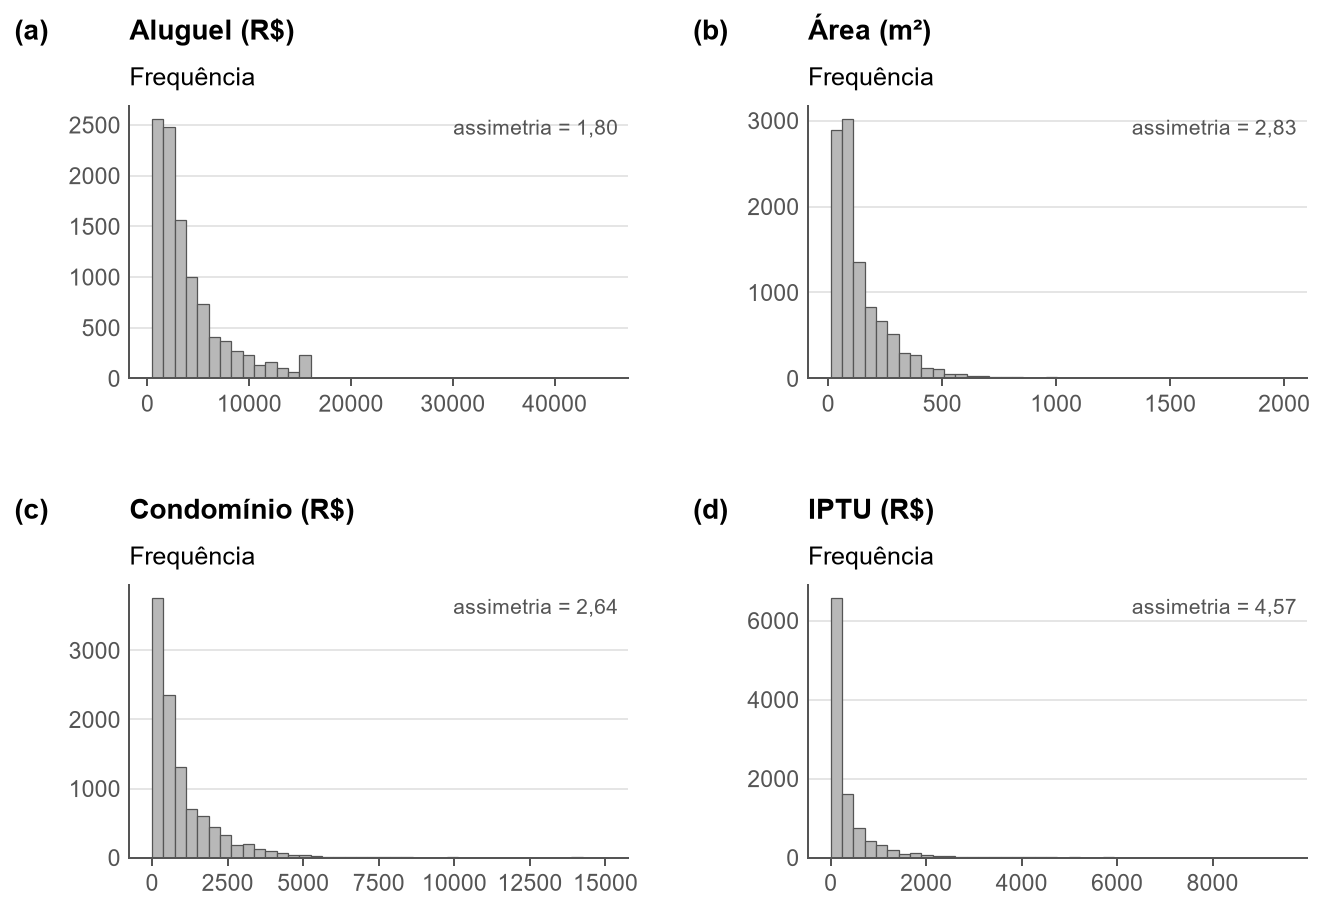
\includegraphics[width=0.88\textwidth]{figuras/hist_originais.png}
\caption{Distribuições das variáveis monetárias e da área na escala original, após a limpeza.}
\label{fig:hist-originais}
\end{figure}
\FloatBarrier

\subsection{Atendimento aos critérios de escolha da base}

A base atende aos três critérios do enunciado: a resposta (aluguel) é contínua; há 11 preditoras candidatas, sendo dez originais, após a exclusão de seguro e total, e a variável derivada \textit{tipo}; e quatro delas são categóricas (cidade, tipo, animal e mobília). Como o número de candidatas é ligeiramente superior a dez, a seleção de variáveis da Seção~\ref{sec:selecao} é aplicada a todas elas.

% =====================================================================
\section{Caracterização das principais variáveis após os tratamentos}

O Bloco~\ref{bl:aed} gera os gráficos da análise exploratória sobre os dados pré-processados e as estatísticas por categoria.

\lstinputlisting[caption={Gráficos e tabelas da análise exploratória.},label={bl:aed}]{codigo/b05_aed.py}

\paragraph{Distribuições.} Na escala $\log_{10}$, o aluguel tem distribuição aproximadamente simétrica (Figura~\ref{fig:hist-transformadas}a), com picos associados a valores arredondados (R\$ 1.500, R\$ 2.000 etc.) e uma concentração no extremo direito, em $\log_{10}(15.000)\approx4{,}18$. Há \textbf{231 anúncios com aluguel exatamente igual a R\$ 15.000} e somente 12 acima desse valor, o que sugere um limite superior na coleta ou no filtro de busca utilizado pelo \textit{crawler}. A documentação da base não menciona esse limite; seu efeito sobre o ajuste é avaliado na Seção~\ref{sec:residuos}. A área em $\log_{10}$ é aproximadamente simétrica. Banheiros, vagas e andar continuam assimétricos, como esperado para contagens, e condomínio e IPTU transformados apresentam o pico em zero discutido anteriormente.

\begin{figure}[H]
\centering
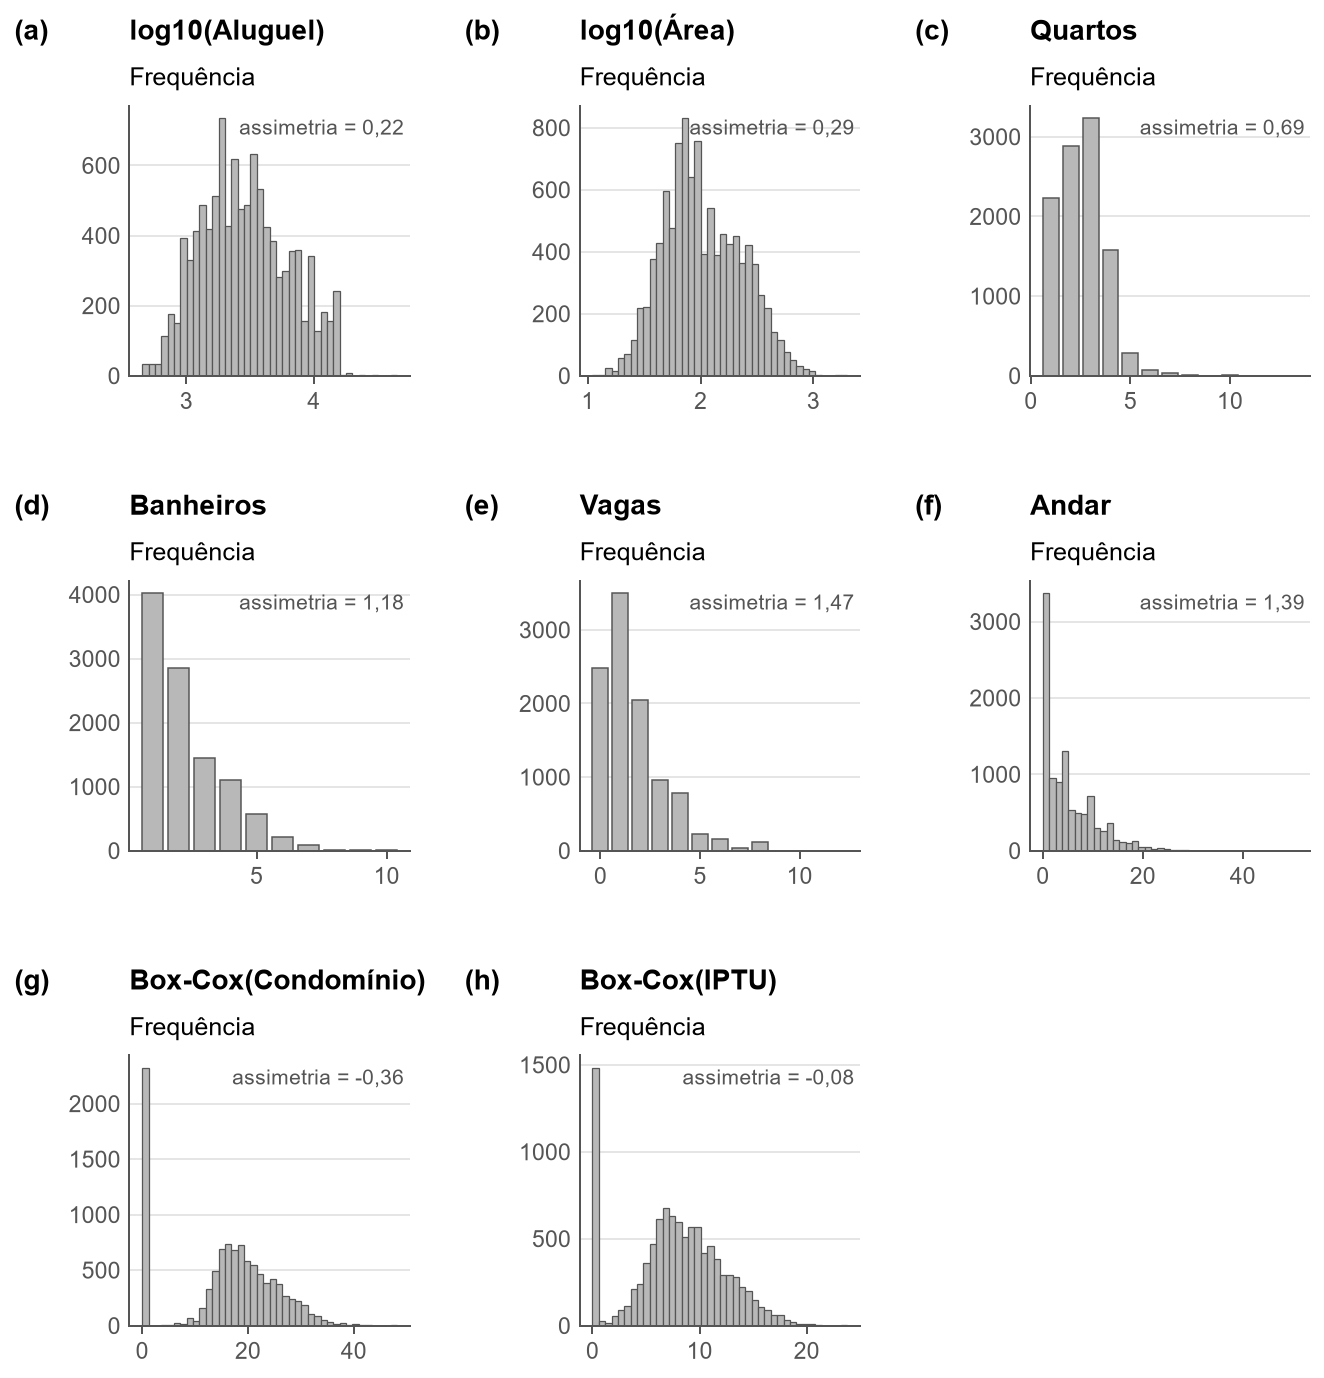
\includegraphics[width=\textwidth]{figuras/hist_transformadas.png}
\caption{Distribuições das variáveis numéricas na escala utilizada no modelo. Contagens são exibidas em gráficos de barras, com uma barra por valor.}
\label{fig:hist-transformadas}
\end{figure}

\paragraph{Variáveis categóricas.} São Paulo concentra 55,3\% dos registros, e a menor categoria é Campinas, com 8,0\% (Figura~\ref{fig:barras}). Há 77,0\% de apartamentos, 78,1\% dos imóveis aceitam animais e 24,3\% são mobiliados. As medianas do aluguel (Figura~\ref{fig:boxplots}) são de R\$ 3.500 em São Paulo, R\$ 2.400 no Rio de Janeiro, R\$ 2.350 em Belo Horizonte, R\$ 1.620 em Porto Alegre e R\$ 1.500 em Campinas. Casas têm mediana maior que apartamentos (R\$ 3.900 e R\$ 2.500), e imóveis mobiliados, maior que não mobiliados (R\$ 3.600 e R\$ 2.460). Essas diferenças são marginais: refletem também diferenças de área e de padrão entre os grupos, e somente o modelo múltiplo permite compará-las com as demais características constantes.

\begin{figure}[H]
\centering
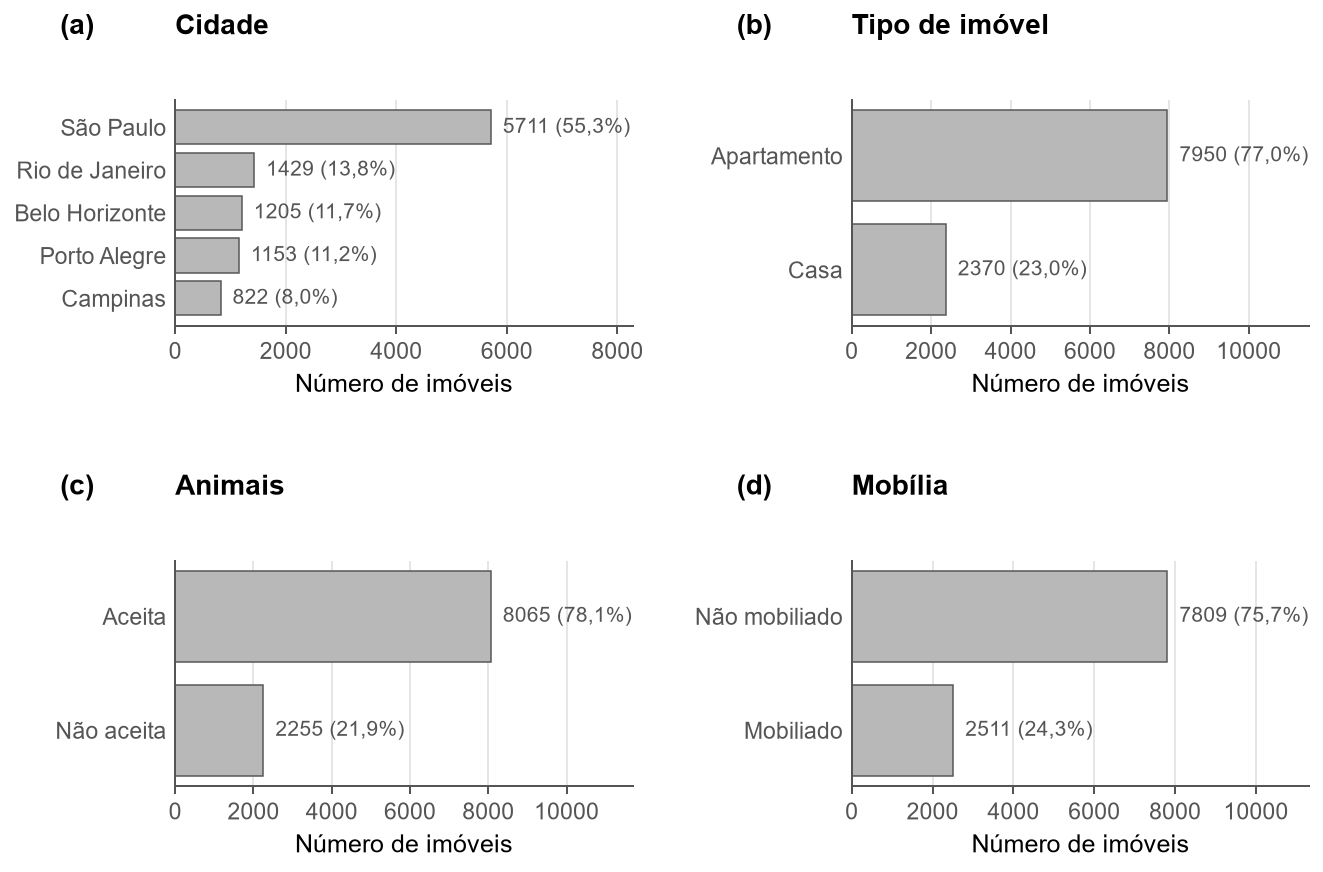
\includegraphics[width=0.92\textwidth]{figuras/barras_categoricas.png}
\caption{Frequências absolutas e relativas das variáveis categóricas.}
\label{fig:barras}
\end{figure}

\begin{figure}[H]
\centering
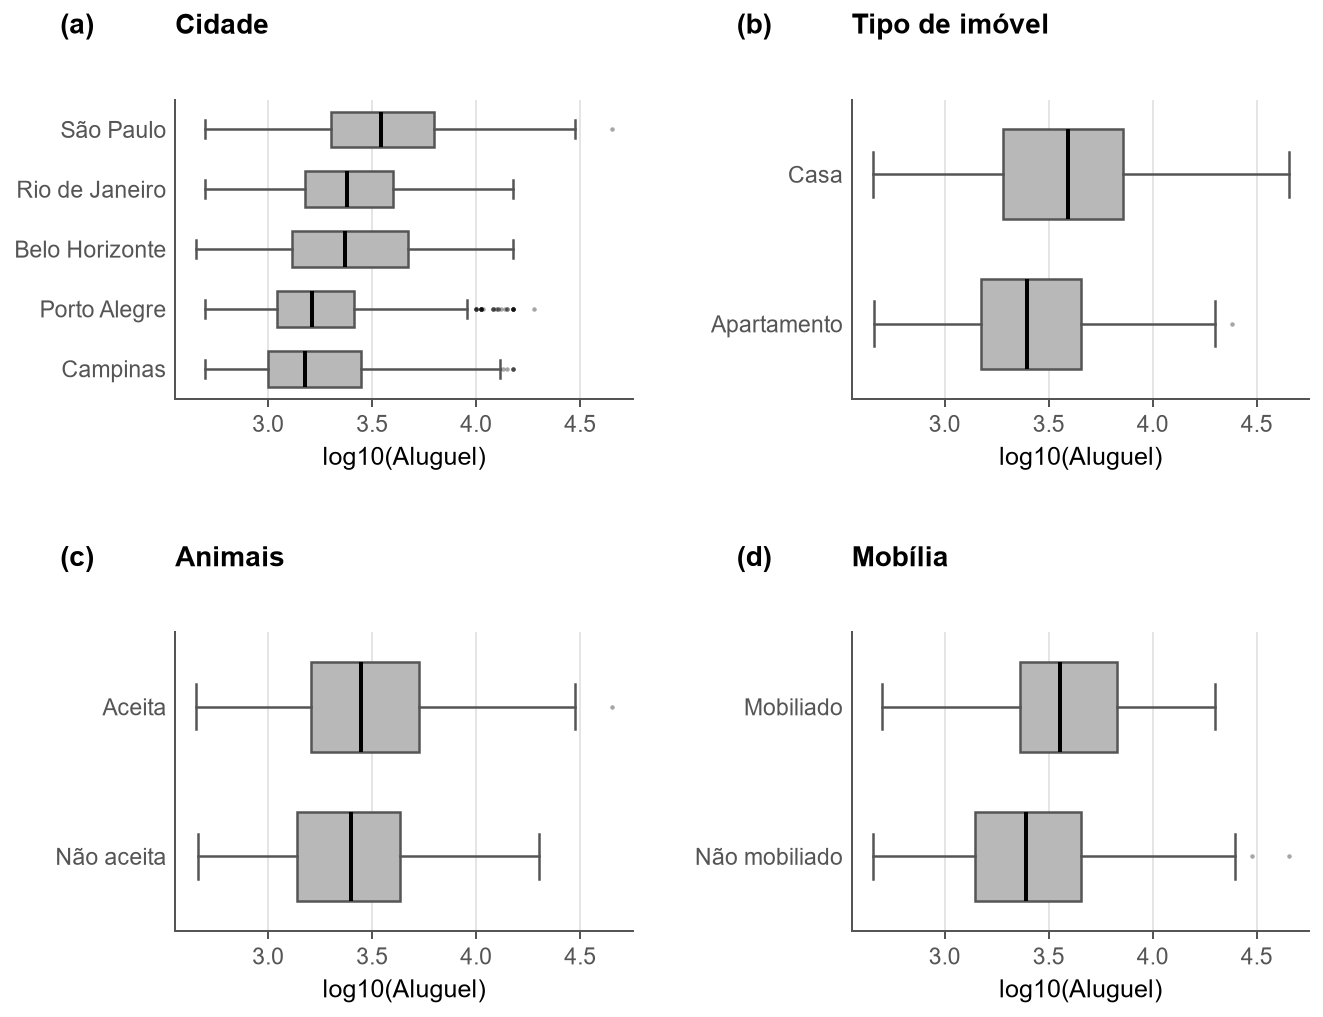
\includegraphics[width=0.92\textwidth]{figuras/boxplots_categoricas.png}
\caption{$\log_{10}(\text{Aluguel})$ por categoria, com categorias ordenadas pela mediana.}
\label{fig:boxplots}
\end{figure}

\paragraph{Associações entre as variáveis numéricas.} A Figura~\ref{fig:matriz} apresenta uma matriz de dispersão adaptada: abaixo da diagonal estão as dispersões de uma amostra de 3.000 registros, com pequeno deslocamento aleatório nas contagens para evitar sobreposição; na diagonal, os histogramas; e acima, os coeficientes de correlação de Pearson calculados com todos os registros. As maiores correlações com $\log_{10}(\text{Aluguel})$ são as de $\log_{10}(\text{Área})$ (0,73), banheiros (0,69), IPTU transformado (0,61), vagas (0,60) e quartos (0,59). As relações são aproximadamente lineares e crescentes.

Entre as preditoras, as variáveis de tamanho são fortemente correlacionadas: a área em escala logarítmica tem correlação de 0,81 com quartos e de 0,80 com banheiros, e quartos e banheiros têm correlação de 0,73. Isso antecipa multicolinearidade e sugere que parte dessas variáveis pode ser redundante. O condomínio transformado tem correlação baixa com o aluguel (0,22), mas a dispersão revela dois grupos: os imóveis sem condomínio, em sua maioria casas, formam uma faixa horizontal em zero, enquanto entre os demais a associação é claramente crescente. A correlação de 0,52 entre andar e condomínio decorre do mesmo fenômeno, pois as casas têm zero nas duas variáveis.

\begin{figure}[H]
\centering
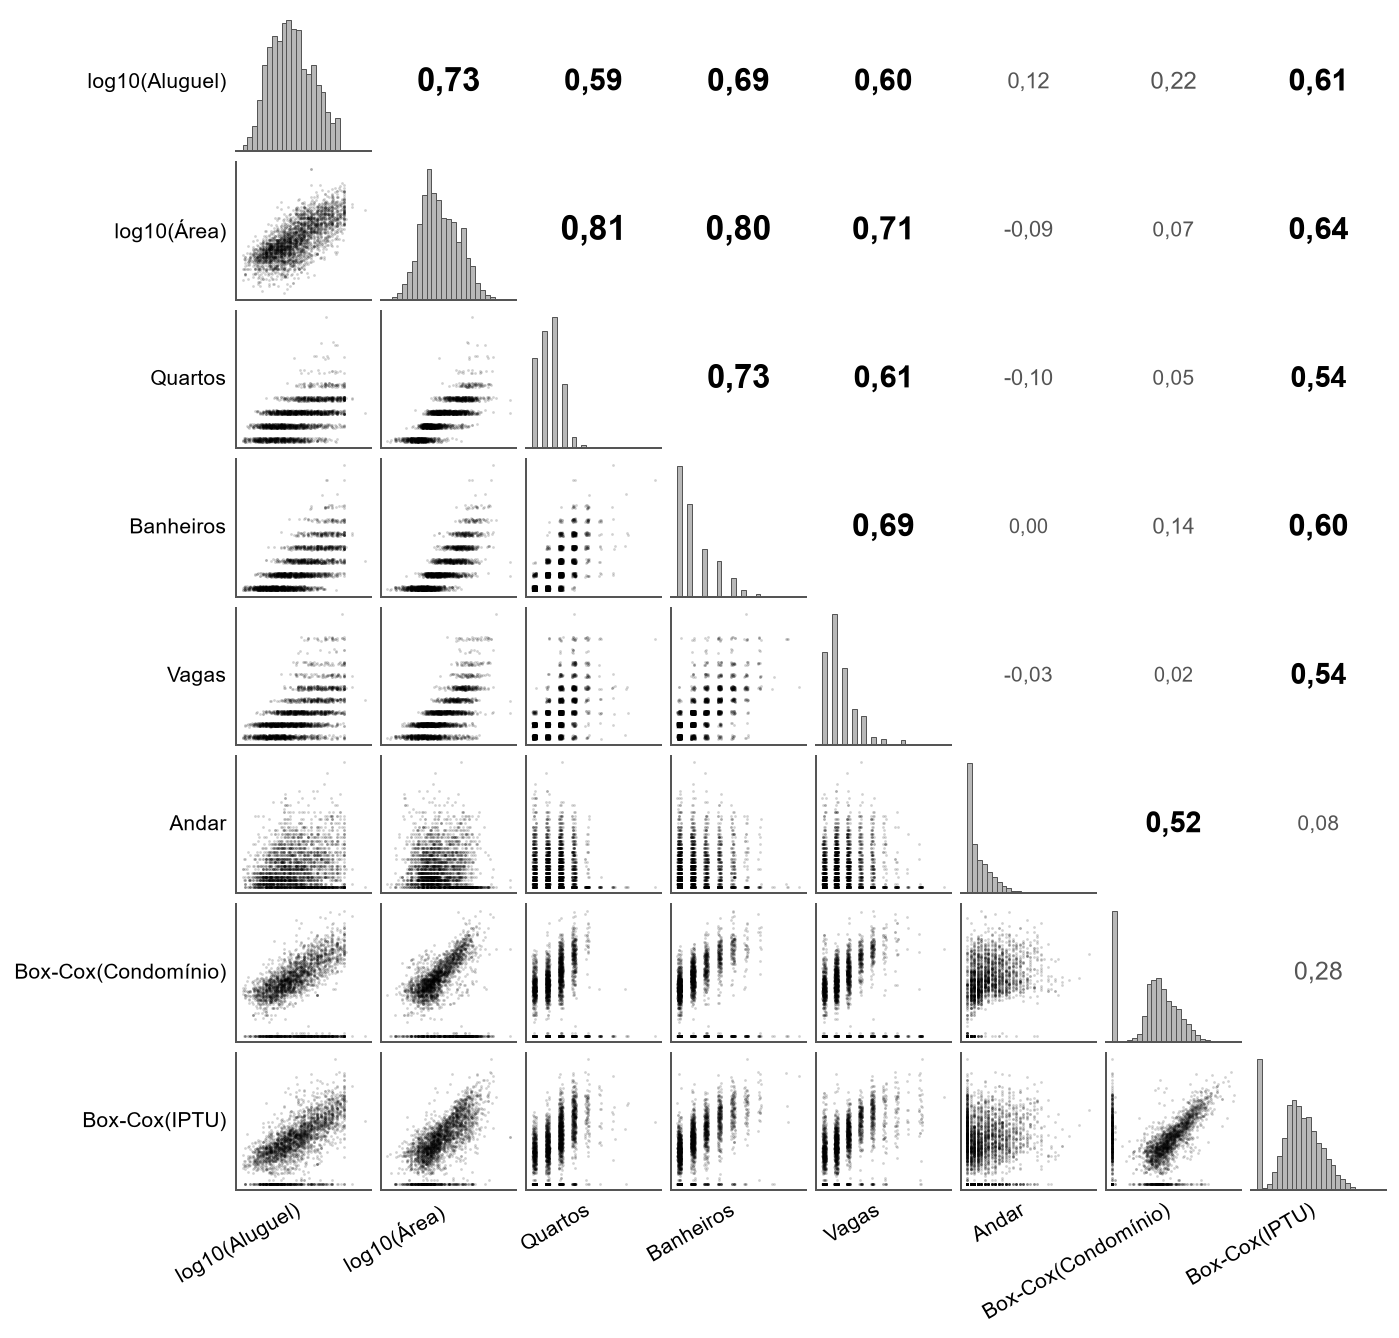
\includegraphics[width=0.86\textwidth]{figuras/matriz_dispersao.png}
\caption{Matriz de dispersão adaptada das variáveis numéricas transformadas: dispersões (abaixo), histogramas (diagonal) e correlações de Pearson (acima; em negrito quando $|r|\geq0{,}5$).}
\label{fig:matriz}
\end{figure}
\FloatBarrier

% =====================================================================
\section{Seleção de variáveis}
\label{sec:selecao}

Foi utilizado o procedimento \textit{stepwise} bidirecional descrito na Lição 10.2 do material STAT 501 \cite{stat501-10}, com níveis $\alpha_E=\alpha_R=0{,}15$ para entrada e remoção. O processo parte do modelo somente com intercepto. Em cada passo, a candidata com menor $p$-valor entra no modelo se $p<\alpha_E$; após cada entrada, os termos já incluídos são reavaliados, e aquele com maior $p$-valor é removido se $p>\alpha_R$. O processo termina quando nenhuma candidata pode entrar e nenhum termo deve sair.

Como \textit{cidade} tem cinco categorias, ela é representada por quatro variáveis indicadoras, que entram ou saem do modelo em conjunto. Por isso, em vez do teste $t$ de um único coeficiente, utilizou-se o teste $F$ parcial, que compara os modelos com e sem o termo e generaliza o teste $t$ para termos com mais de um grau de liberdade. Com $n=10.320$, alguns $p$-valores ficam abaixo do menor número representável em ponto flutuante e são arredondados para zero. Por esse motivo, a ordenação das candidatas foi feita pelo logaritmo do $p$-valor.

\lstinputlisting[caption={Seleção \textit{stepwise} por teste $F$ parcial.},label={bl:stepwise}]{codigo/b06_stepwise.py}

\begin{table}[H]
\centering
\caption{Trajetória do \textit{stepwise} ($\alpha_E=\alpha_R=0{,}15$). Nenhum termo foi removido após entrar.}
\label{tab:stepwise}
\footnotesize
\begin{tabular}{clllrrr}
\toprule
Passo & Ação & Termo & gl & $F$ parcial & $p$-valor & \Rtwoadj{} após \\
\midrule
1 & Entrada & $\log_{10}(\text{Área})$ & 1 & 11.631,34 & $<10^{-300}$ & 0,5299 \\
2 & Entrada & Cidade & 4 & 454,17 & $<10^{-300}$ & 0,6001 \\
3 & Entrada & Mobília & 1 & 1.286,62 & $1{,}222\times10^{-265}$ & 0,6444 \\
4 & Entrada & Banheiros & 1 & 605,27 & $6{,}356\times10^{-130}$ & 0,6641 \\
5 & Entrada & BC(IPTU) & 1 & 423,48 & $3{,}003\times10^{-92}$ & 0,6773 \\
6 & Entrada & Andar & 1 & 301,31 & $1{,}504\times10^{-66}$ & 0,6865 \\
7 & Entrada & Vagas & 1 & 83,85 & $6{,}364\times10^{-20}$ & 0,6890 \\
8 & Entrada & BC(Condomínio) & 1 & 19,15 & $1{,}217\times10^{-5}$ & 0,6895 \\
9 & Entrada & Tipo & 1 & 41,81 & $1{,}052\times10^{-10}$ & 0,6907 \\
10 & Entrada & Animais & 1 & 8,65 & 0,0033 & 0,6910 \\
\bottomrule
\end{tabular}

\end{table}

A Tabela~\ref{tab:stepwise} mostra que dez termos entraram, na ordem de sua contribuição incremental, e nenhum foi removido. A área entra primeiro e, sozinha, produz \Rtwoadj$=0{,}5299$; cidade e mobília elevam esse valor para 0,6444. \textbf{Quartos foi a única candidata não selecionada}: com os demais termos no modelo, o teste $F$ parcial para sua inclusão resulta em $p=0{,}9568$. Esse resultado é coerente com a Figura~\ref{fig:matriz}: dadas a área e o número de banheiros, o número de quartos não acrescenta informação sobre o aluguel, pois, para uma área fixa, mais quartos significam apenas cômodos menores.

\begin{table}[H]
\centering
\caption{Comparação entre o modelo com todas as candidatas e o modelo selecionado.}
\label{tab:comparacao}
\footnotesize
\begin{tabular}{lrrrrrr}
\toprule
Modelo & Termos & Parâmetros & \Rtwo{} & \Rtwoadj{} & AIC & BIC \\
\midrule
Completo & 11 & 15 & 0,6914 & 0,6909 & -4.908,20 & -4.799,57 \\
Selecionado & 10 & 14 & 0,6914 & 0,6910 & -4.910,20 & -4.808,81 \\
\midrule
\multicolumn{7}{l}{\footnotesize Teste $F$ parcial para incluir Quartos: $F=0,0029$; $p=0,9568$.}\\
\bottomrule
\end{tabular}

\end{table}

Os critérios de informação concordam com o \textit{stepwise}: AIC e BIC são menores no modelo selecionado (Tabela~\ref{tab:comparacao}), e a remoção de quartos não altera o \Rtwo{} até a quarta casa decimal.

Com mais de dez mil observações, porém, efeitos muito pequenos já são estatisticamente significativos: Animais entrou com $p=0{,}0033$, mas elevou o \Rtwoadj{} em apenas 0,0002. Para avaliar a relevância prática de cada termo, a Tabela~\ref{tab:importancia} apresenta a queda no \Rtwo{} quando o termo é retirado do modelo selecionado. Área, cidade e mobília dominam; os outros sete termos, isoladamente, contribuem com menos de 0,01 cada. A soma das contribuições é menor que o \Rtwo{} total porque parte da variabilidade explicada é compartilhada entre preditoras correlacionadas. O modelo selecionado foi mantido como modelo final, conforme o critério estabelecido, mas a interpretação dos efeitos considera também sua magnitude.

\begin{table}[H]
\centering
\caption{Contribuição de cada termo: redução do \Rtwo{} ao retirá-lo do modelo selecionado.}
\label{tab:importancia}
\footnotesize
\begin{tabular}{lrrr}
\toprule
Termo & gl & $\Delta R^2$ ao remover & \% do \Rtwo{} \\
\midrule
$\log_{10}(\text{Área})$ & 1 & 0,0495 & 7,2 \\
Cidade & 4 & 0,0377 & 5,5 \\
Mobília & 1 & 0,0300 & 4,3 \\
Banheiros & 1 & 0,0078 & 1,1 \\
BC(IPTU) & 1 & 0,0066 & 1,0 \\
Andar & 1 & 0,0061 & 0,9 \\
Vagas & 1 & 0,0026 & 0,4 \\
BC(Condomínio) & 1 & 0,0018 & 0,3 \\
Tipo & 1 & 0,0012 & 0,2 \\
Animais & 1 & 0,0003 & 0,0 \\
\bottomrule
\end{tabular}

\end{table}
\FloatBarrier

% =====================================================================
\section{Resultados e discussões}

\subsection{Coeficientes do modelo selecionado}

O modelo final foi ajustado por mínimos quadrados ordinários (OLS), com estimativa clássica, não robusta, da matriz de covariância dos coeficientes (Bloco~\ref{bl:modelo}). Os intervalos dos coeficientes foram calculados por $\widehat{\beta}_j\pm t_{0,975;\,n-p}\,\mathrm{EP}(\widehat{\beta}_j)$, com $p=14$ parâmetros. Como na Atividade 1, os $p$-valores e os intervalos são \textbf{nominais}: sua validade depende das premissas avaliadas nas próximas subseções.

\lstinputlisting[caption={Ajuste do modelo final e efeitos na escala original.},label={bl:modelo}]{codigo/b07_modelo_final.py}

\begin{table}[H]
\centering
\caption{Coeficientes do modelo final, com IC nominais de 95\%. Resposta: $\log_{10}(\text{Aluguel})$; referências: São Paulo, Apartamento, Não mobiliado e Aceita.}
\label{tab:coeficientes}
\footnotesize
\begin{tabular}{lrrrrl}
\toprule
Termo & Estimativa & EP & $t$ & $p$-valor & IC 95\% \\
\midrule
Intercepto & 2,31109 & 0,01737 & 133,062 & $<0,0001$ & [2,27704; 2,34513] \\
Cidade: Rio de Janeiro & -0,03571 & 0,00593 & -6,022 & $<0,0001$ & [-0,04733; -0,02408] \\
Cidade: Belo Horizonte & -0,11683 & 0,00627 & -18,648 & $<0,0001$ & [-0,12911; -0,10455] \\
Cidade: Porto Alegre & -0,14509 & 0,00640 & -22,666 & $<0,0001$ & [-0,15764; -0,13254] \\
Cidade: Campinas & -0,20240 & 0,00721 & -28,085 & $<0,0001$ & [-0,21653; -0,18828] \\
Tipo: Casa & 0,05469 & 0,00860 & 6,356 & $<0,0001$ & [0,03782; 0,07155] \\
Mobília: Mobiliado & 0,14230 & 0,00450 & 31,651 & $<0,0001$ & [0,13349; 0,15112] \\
Animais: Não aceita & 0,01373 & 0,00467 & 2,941 & 0,0033 & [0,00458; 0,02288] \\
$\log_{10}(\text{Área})$ & 0,44291 & 0,01089 & 40,665 & $<0,0001$ & [0,42156; 0,46426] \\
Banheiros & 0,03838 & 0,00237 & 16,163 & $<0,0001$ & [0,03373; 0,04304] \\
Vagas & 0,01687 & 0,00181 & 9,340 & $<0,0001$ & [0,01333; 0,02042] \\
Andar & 0,00616 & 0,00043 & 14,237 & $<0,0001$ & [0,00531; 0,00701] \\
BC(Condomínio) & 0,00271 & 0,00035 & 7,673 & $<0,0001$ & [0,00202; 0,00340] \\
BC(IPTU) & 0,00871 & 0,00059 & 14,854 & $<0,0001$ & [0,00756; 0,00985] \\
\bottomrule
\end{tabular}

\end{table}

O modelo ajustado é
\begin{multline*}
  \widehat{\log_{10}(\textit{aluguel})} = 2{,}3111
  - 0{,}0357\,\text{RJ} - 0{,}1168\,\text{BH} - 0{,}1451\,\text{POA} - 0{,}2024\,\text{CPS} \\
  + 0{,}0547\,\text{Casa} + 0{,}1423\,\text{Mobiliado} + 0{,}0137\,\text{NãoAceita}
  + 0{,}4429\log_{10}(\textit{area}) \\
  + 0{,}0384\,\textit{banheiros} + 0{,}0169\,\textit{vagas} + 0{,}0062\,\textit{andar} \\
  + 0{,}0027\,\mathrm{BC}(\textit{condominio}) + 0{,}0087\,\mathrm{BC}(\textit{iptu}),
\end{multline*}
em que RJ, BH, POA, CPS, Casa, Mobiliado e NãoAceita são variáveis indicadoras e $\mathrm{BC}(\cdot)$ denota a transformação Box-Cox de $X+1$ com os $\lambda^*$ da Tabela~\ref{tab:boxcox}. Todos os coeficientes têm IC de 95\% que não contém zero (Tabela~\ref{tab:coeficientes}).

Como a resposta está em $\log_{10}$, um acréscimo $b$ no preditor linear corresponde a multiplicar o aluguel por $10^{b}$. Sob erros normais na escala logarítmica, $10^{\widehat{y}}$ estima a \textbf{mediana condicional} do aluguel, e não diretamente sua média, assim como na Atividade 1. A Tabela~\ref{tab:efeitos} converte os coeficientes em variações percentuais dessa mediana, mantidas as demais variáveis constantes.

\begin{table}[H]
\centering
\caption{Efeitos estimados na escala original: variação percentual da mediana condicional do aluguel, com as demais variáveis constantes.}
\label{tab:efeitos}
\footnotesize
\begin{tabular}{llrl}
\toprule
Termo & Comparação & Variação (\%) & IC 95\% (\%) \\
\midrule
Cidade: Rio de Janeiro & vs. referência & -7,9 & [-10,3; -5,4] \\
Cidade: Belo Horizonte & vs. referência & -23,6 & [-25,7; -21,4] \\
Cidade: Porto Alegre & vs. referência & -28,4 & [-30,4; -26,3] \\
Cidade: Campinas & vs. referência & -37,3 & [-39,3; -35,2] \\
Tipo: Casa & vs. referência & 13,4 & [9,1; 17,9] \\
Mobília: Mobiliado & vs. referência & 38,8 & [36,0; 41,6] \\
Animais: Não aceita & vs. referência & 3,2 & [1,1; 5,4] \\
$\log_{10}(\text{Área})$ & +10\% de área & 4,3 & [4,1; 4,5] \\
Banheiros & +1 banheiro & 9,2 & [8,1; 10,4] \\
Vagas & +1 vaga & 4,0 & [3,1; 4,8] \\
Andar & +1 andar & 1,4 & [1,2; 1,6] \\
BC(Condomínio) & 1.º $\to$ 3.º quartil & 7,1 & [5,2; 9,0] \\
BC(IPTU) & 1.º $\to$ 3.º quartil & 11,6 & [10,0; 13,3] \\
\bottomrule
\end{tabular}

\end{table}

\begin{itemize}
  \item \textbf{Cidade:} para imóveis com as mesmas características, o aluguel mediano é 7,9\% menor no Rio de Janeiro do que em São Paulo, 23,6\% menor em Belo Horizonte, 28,4\% menor em Porto Alegre e 37,3\% menor em Campinas.
  \item \textbf{Mobília:} imóveis mobiliados têm aluguel mediano 38,8\% maior, o maior efeito entre as variáveis binárias.
  \item \textbf{Área:} como resposta e preditora estão em $\log_{10}$, o coeficiente 0,443 é uma elasticidade. Um aumento de 10\% na área está associado a um aluguel 4,3\% maior, e dobrar a área multiplica o aluguel mediano por $2^{0{,}443}\approx1{,}36$. O aluguel cresce menos que proporcionalmente à área; portanto, o valor por metro quadrado diminui à medida que o imóvel aumenta.
  \item \textbf{Banheiros, vagas e andar:} cada banheiro adicional está associado a um aumento de 9,2\%, cada vaga a 4,0\%, e cada andar a 1,4\%, o que corresponde a cerca de 15\% entre o 1.º e o 11.º andar.
  \item \textbf{Tipo:} a estimativa de 13,4\% compara uma casa com um apartamento hipotético no andar 0. Em relação a um apartamento no 1.º andar, a diferença é $10^{0{,}0547-0{,}0062}-1\approx11{,}8\%$.
  \item \textbf{Condomínio e IPTU:} como as escalas Box-Cox não têm interpretação direta, comparou-se o 1.º com o 3.º quartil de cada variável original. Passar de um condomínio de R\$ 180 para R\$ 1.283 está associado a um aluguel 7,1\% maior; passar de um IPTU de R\$ 40 para R\$ 386, a um aluguel 11,6\% maior. Como o IPTU é calculado sobre o valor venal do imóvel, essas variáveis provavelmente capturam parte do efeito da localização e do padrão do imóvel, que não estão na base.
  \item \textbf{Animais:} não aceitar animais está associado a um aluguel 3,2\% maior. O efeito é estatisticamente significativo, mas pequeno, e pode refletir características não observadas, como edifícios de padrão mais alto com regras mais restritivas.
\end{itemize}

O intercepto corresponde a um imóvel de 1 m$^2$, sem banheiros, vagas, condomínio ou IPTU, situação fora da faixa observada; por isso, não tem interpretação direta. Os efeitos descritos são \textbf{associações condicionais} em dados observacionais, e não efeitos causais.

\subsection{Coeficiente de determinação e teste F}

\begin{table}[H]
\centering
\caption{ANOVA do modelo final.}
\label{tab:anova}
\small
\begin{tabular}{lrrrrr}
\toprule
Fonte & gl & SQ & QM & $F$ & $p$-valor \\
\midrule
Regressão & 13 & 838,780 & 64,5215 & 1.775,83 & $<0,0001$ \\
Resíduos & 10.306 & 374,449 & 0,03633 & \NA & \NA \\
Total & 10.319 & 1.213,228 & \NA & \NA & \NA \\
\midrule
\multicolumn{6}{l}{\footnotesize $S=0,1906$; \Rtwo$=0,6914$; \Rtwoadj$=0,6910$.}\\
\bottomrule
\end{tabular}

\end{table}

\begin{table}[H]
\centering
\caption{Resumo OLS do modelo final.}
\label{tab:resumo}
\small
\begin{tabular}{lrlr}
\toprule
Estatística & Valor & Estatística & Valor \\
\midrule
Observações & 10.320 & gl modelo/resíduos & 13/10.306 \\
\Rtwo{} & 0,6914 & \Rtwoadj{} & 0,6910 \\
$F$ & 1.775,83 & $p(F)$ & $<10^{-300}$ \\
Log-verossimilhança & 2.469,098 & AIC & -4.910,197 \\
BIC & -4.808,811 & Número de condição & 227,9 \\
Omnibus & 159,097 & $p(\text{Omnibus})$ & $2{,}835\times10^{-35}$ \\
JB & 270,283 & $p(\text{JB})$ & $2{,}036\times10^{-59}$ \\
Assimetria & 0,121 & Curtose & 3,755 \\
DW (ordem do arquivo) & 2,036 & Covariância & Clássica \\
\bottomrule
\end{tabular}

\end{table}

O modelo explica \textbf{69,14\%} da variabilidade amostral de $\log_{10}(\text{Aluguel})$ (\Rtwo$=0{,}6914$), com \Rtwoadj$=0{,}6910$ (Tabelas~\ref{tab:anova} e \ref{tab:resumo}). Os dois valores são praticamente iguais porque $n$ é muito maior que o número de parâmetros. Essa porcentagem se refere ao logaritmo do aluguel, não ao aluguel em reais.

O teste $F$ de significância global resulta em $F(13;\,10.306)=1.775{,}83$, com $p<10^{-300}$. Rejeita-se, portanto, a hipótese nula de que todos os coeficientes, exceto o intercepto, sejam nulos, ressalvada a natureza nominal do teste. O erro padrão residual é $S=0{,}1906$ na escala $\log_{10}$. Sob normalidade, cerca de 68\% dos aluguéis estariam entre $10^{-S}\approx0{,}64$ e $10^{S}\approx1{,}55$ vezes a mediana prevista, isto é, de 36\% abaixo a 55\% acima. Essa largura mostra que, embora o modelo explique uma fração importante da variabilidade, o erro de previsão para um imóvel individual permanece considerável.

\subsection{Gráficos dos resíduos}
\label{sec:residuos}

O Bloco~\ref{bl:graficos-residuos} gera os gráficos de diagnóstico e resume os resíduos por cidade e por decil dos valores preditos.

\lstinputlisting[caption={Gráficos dos resíduos e resíduos por faixa de valores preditos.},label={bl:graficos-residuos}]{codigo/b08_graficos_residuos.py}

\begin{figure}[H]
\centering
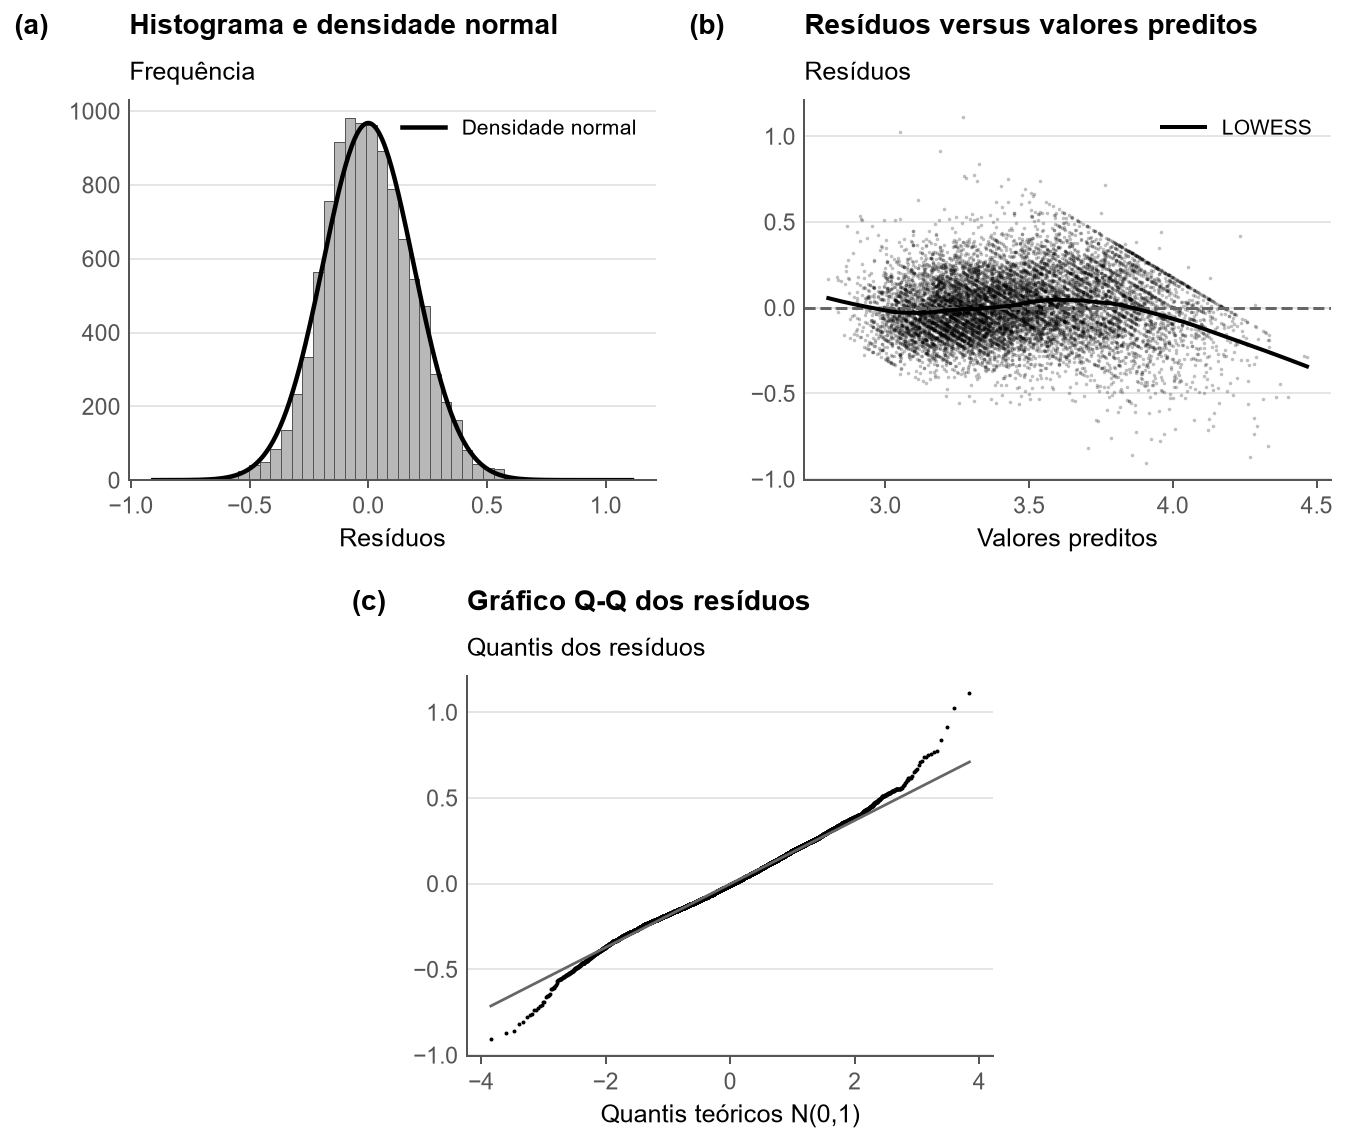
\includegraphics[width=0.9\textwidth]{figuras/diagnostico_final.png}
\caption{Diagnóstico do modelo final: (a) histograma com densidade normal de referência; (b) resíduos versus valores preditos, com curva LOWESS; (c) gráfico Q--Q.}
\label{fig:diagnostico}
\end{figure}

\paragraph{Histograma e Q--Q.} O histograma (Figura~\ref{fig:diagnostico}a) é unimodal, aproximadamente simétrico e acompanha bem a densidade normal, com pico um pouco mais alto e caudas um pouco mais pesadas (assimetria de 0,121 e curtose de 3,755; na normal, 0 e 3). No Q--Q (Figura~\ref{fig:diagnostico}c), os pontos seguem a reta de referência na região central e se afastam dela nas duas caudas, sobretudo na superior. O maior resíduo, 1,11, corresponde a um aluguel observado cerca de 13 vezes maior que a mediana prevista. A fração de resíduos com $|e_i|>2S$ é de 4,48\%, próxima dos 4,55\% esperados sob normalidade.

\paragraph{Resíduos versus preditos.} Na Figura~\ref{fig:diagnostico}b, a nuvem está centrada em zero em quase toda a faixa de valores preditos, sem um funil pronunciado. As faixas diagonais decorrem do arredondamento dos aluguéis (R\$ 1.500, R\$ 2.000 etc.): para um valor observado fixo $y$, o resíduo $y-\widehat{y}$ diminui linearmente com $\widehat{y}$. Trata-se de um efeito da discretização da resposta, e não de uma falha do modelo. A faixa mais visível, que forma a borda superior da nuvem à direita, corresponde ao aluguel de R\$ 15.000. A curva LOWESS fica levemente abaixo de zero entre cerca de 3,0 e 3,3, levemente acima entre 3,5 e 3,8 e decresce a partir de cerca de 3,9, isto é, de aproximadamente R\$ 8 mil.

\begin{table}[H]
\centering
\caption{Resíduos por decil dos valores preditos.}
\label{tab:decis}
\footnotesize
\begin{tabular}{crrrrr}
\toprule
Decil & Predito médio & $10^{\text{predito}}$ (R\$) & Média res. & DP res. & \% com aluguel $\geq$ R\$ 15 mil \\
\midrule
1 & 3,037 & 1.089 & -0,0222 & 0,1659 & 0,0 \\
2 & 3,162 & 1.451 & -0,0228 & 0,1636 & 0,0 \\
3 & 3,239 & 1.734 & -0,0180 & 0,1669 & 0,1 \\
4 & 3,311 & 2.045 & -0,0075 & 0,1754 & 0,0 \\
5 & 3,385 & 2.427 & 0,0031 & 0,1803 & 0,0 \\
6 & 3,466 & 2.924 & 0,0197 & 0,1870 & 0,3 \\
7 & 3,556 & 3.594 & 0,0470 & 0,1957 & 0,6 \\
8 & 3,662 & 4.596 & 0,0420 & 0,2050 & 1,6 \\
9 & 3,792 & 6.196 & 0,0251 & 0,2151 & 5,1 \\
10 & 3,995 & 9.895 & -0,0664 & 0,2131 & 15,8 \\
\bottomrule
\end{tabular}

\end{table}

A Tabela~\ref{tab:decis} quantifica esse padrão. A média dos resíduos é de cerca de $-0{,}02$ nos três primeiros decis, chega a $+0{,}047$ no sétimo e cai para $-0{,}066$ no décimo, decil em que 15,8\% dos anúncios têm aluguel de R\$ 15.000 ou mais. Nesse decil, o aluguel observado é, em média, cerca de 14\% menor que a mediana prevista ($10^{-0{,}066}\approx0{,}86$). A explicação mais provável é o \textbf{teto aparente da coleta}: para imóveis grandes e caros, o aluguel observado fica limitado a cerca de R\$ 15.000, enquanto o modelo prolonga a tendência linear. Isso produz um desvio sistemático de L no extremo superior. Nos demais decis, os desvios de linearidade são pequenos. O desvio padrão dos resíduos cresce de 0,164 nos primeiros decis para 0,215 no nono, o que corresponde a uma variância cerca de 1,7 vez maior nas faixas superiores; esse resultado é retomado na avaliação de E.

\begin{figure}[H]
\centering
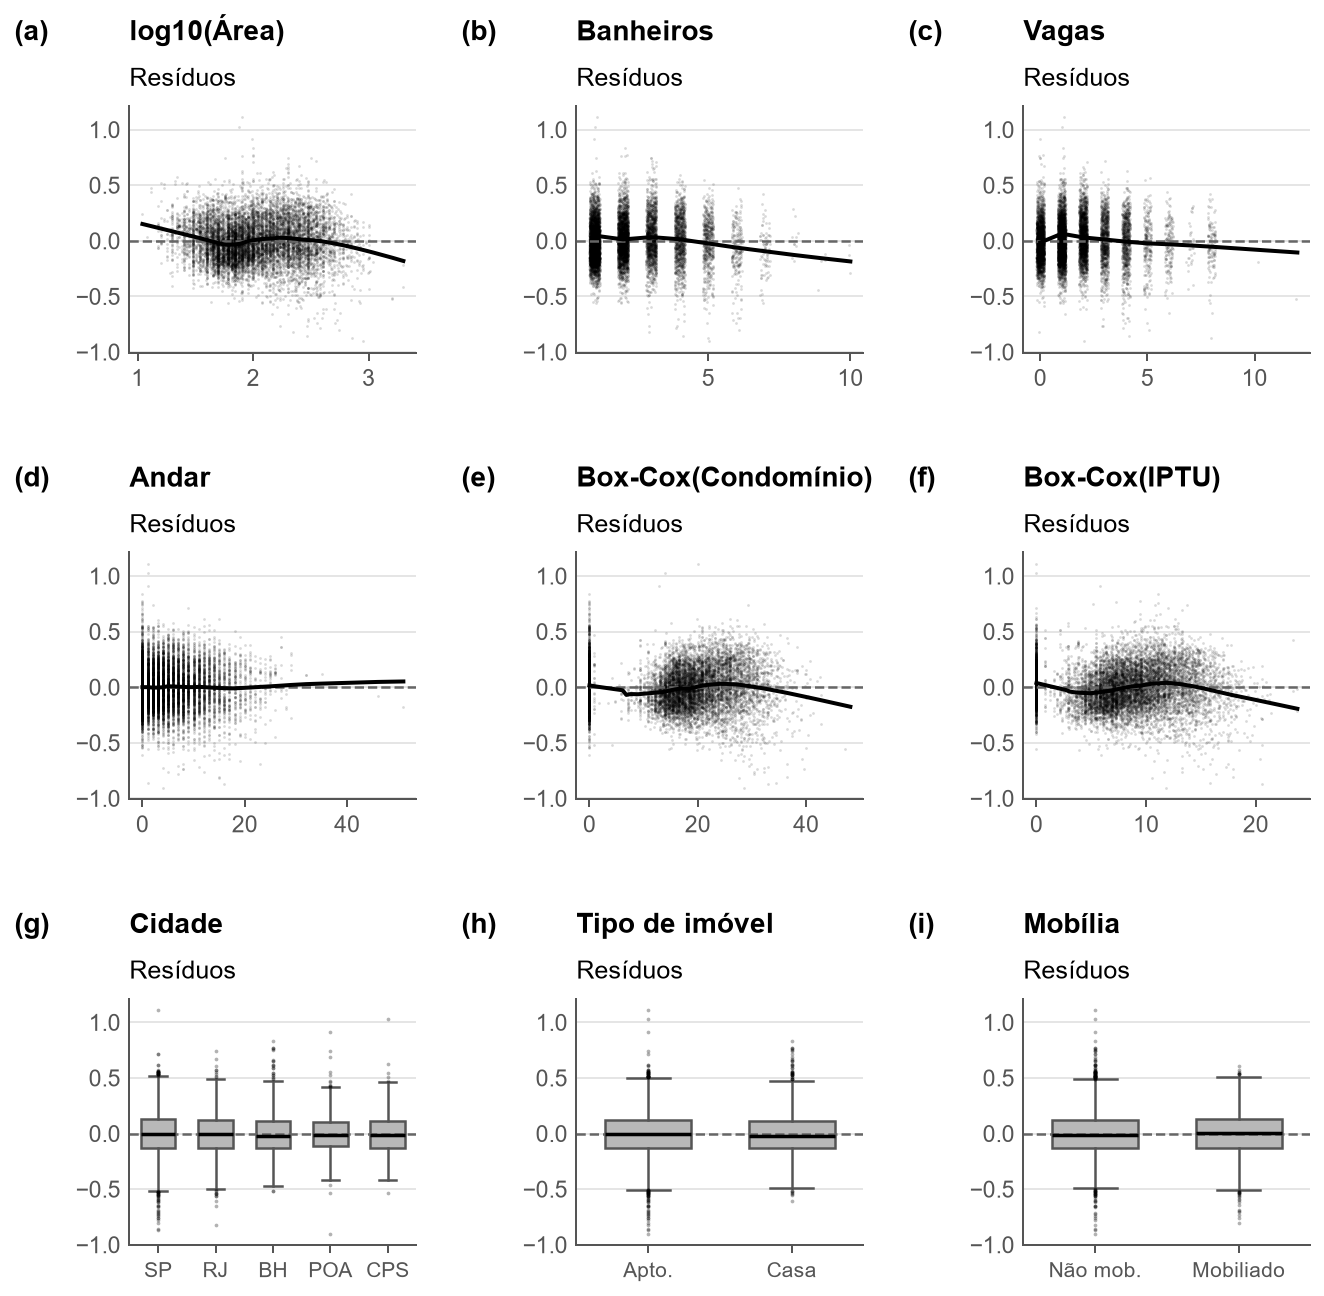
\includegraphics[width=\textwidth]{figuras/residuos_preditores.png}
\caption{Resíduos versus cada preditora selecionada, com curva LOWESS para as numéricas (a)--(f) e boxplots para as categóricas (g)--(i). SP: São Paulo; RJ: Rio de Janeiro; BH: Belo Horizonte; POA: Porto Alegre; CPS: Campinas.}
\label{fig:residuos-preditores}
\end{figure}

\paragraph{Resíduos versus preditoras.} Nos gráficos contra cada preditora (Figura~\ref{fig:residuos-preditores}), as curvas LOWESS permanecem próximas de zero na região em que se concentra a grande maioria dos registros, o que dá suporte à forma linear adotada para cada variável. Os desvios aparecem nos extremos, onde há poucos dados: imóveis pequenos (abaixo de cerca de 40 m$^2$, isto é, $\log_{10}(\text{Área})<1{,}6$) têm resíduos positivos, compatíveis com um preço por metro quadrado maior em quitinetes e estúdios; imóveis muito grandes, com muitos banheiros ou com condomínio e IPTU altos têm resíduos negativos, o mesmo padrão associado ao teto de R\$ 15.000. Nas variáveis categóricas, a média dos resíduos é zero em todas as categorias por construção, pois cada categoria tem sua própria indicadora, mas a dispersão varia: o desvio padrão dos resíduos é de 0,164 em Porto Alegre e de 0,174 em Campinas, contra 0,197 em São Paulo.

\subsection{Testes estatísticos sobre os resíduos}

O Bloco~\ref{bl:testes} aplica cinco testes de normalidade e três testes de homogeneidade das variâncias. No teste de Goldfeld--Quandt, os registros foram ordenados pelos valores preditos, e os 20\% centrais foram descartados, comparando-se as variâncias residuais dos 40\% inferiores e dos 40\% superiores. O teste de Brown--Forsythe, versão do teste de Levene baseada na mediana, compara as variâncias dos resíduos entre as cidades.

\lstinputlisting[caption={Testes de normalidade e de homogeneidade das variâncias dos resíduos.},label={bl:testes}]{codigo/b09_testes_residuos.py}

\begin{table}[H]
\centering
\caption{Testes sobre os resíduos do modelo final ($n=10.320$).}
\label{tab:testes}
\small
\begin{tabular}{llrr}
\toprule
Premissa & Teste & Estatística & $p$-valor \\
\midrule
Normalidade & Shapiro--Wilk & 0,9948 & $7{,}267\times10^{-19}$ \\
Normalidade & Kolmogorov--Smirnov (Lilliefors) & 0,0212 & $\le 0,001$ \\
Normalidade & Anderson--Darling & 9,0315 & $6{,}709\times10^{-22}$ \\
Normalidade & Jarque--Bera & 270,2826 & $2{,}036\times10^{-59}$ \\
Normalidade & D'Agostino--Pearson (Omnibus) & 159,0967 & $2{,}835\times10^{-35}$ \\
\addlinespace
Variância & Breusch--Pagan (Koenker) & 216,2812 & $6{,}100\times10^{-39}$ \\
Variância & Goldfeld--Quandt (preditos) & 1,5634 & $3{,}237\times10^{-42}$ \\
Variância & Brown--Forsythe (cidades) & 15,8176 & $6{,}517\times10^{-13}$ \\
\bottomrule
\end{tabular}

\end{table}

\paragraph{Normalidade.} Todos os testes rejeitam a normalidade dos resíduos (Tabela~\ref{tab:testes}). Com $n=10.320$, porém, esses testes detectam desvios muito pequenos; o resultado deve ser lido em conjunto com a magnitude do desvio, que é pequena: assimetria de 0,121, curtose de 3,755 e uma fração de resíduos acima de $2S$ praticamente igual à esperada. O desvio concentra-se nas caudas, como mostrou o Q--Q. A SciPy alerta que o $p$-valor de Shapiro--Wilk pode ser impreciso para $n>5.000$, por isso ele é apresentado apenas como complemento; o $p$-valor de Lilliefors é obtido de uma tabela e truncado em 0,001. Conclui-se que N não é estritamente satisfeita, mas a violação é leve. Para a inferência sobre os coeficientes, com esse tamanho amostral, o teorema central do limite torna os intervalos aproximadamente válidos; para intervalos de predição de aluguéis individuais, as caudas mais pesadas podem comprometer a cobertura nominal nos extremos.

\paragraph{Homogeneidade das variâncias.} Os três testes rejeitam a homocedasticidade. Na estatística de Goldfeld--Quandt, $F=1{,}563$ indica que a variância residual nos 40\% maiores valores preditos é 56\% maior que nos 40\% menores, e o teste de Brown--Forsythe confirma variâncias diferentes entre as cidades. Assim, E \textbf{não é satisfeita}; a heterocedasticidade é moderada, sem o funil acentuado do modelo na escala original (Seção~\ref{sec:comparacao}). Sua consequência sobre os erros padrão é avaliada a seguir.

\paragraph{Independência.} A estatística de Durbin--Watson calculada na ordem do arquivo é 2,036. Como os dados são transversais e a ordem do arquivo não corresponde a uma sequência temporal de coleta, esse valor não é usado para declarar independência.

\subsection{Multicolinearidade, observações influentes e erros padrão robustos}

O Bloco~\ref{bl:influencia} calcula os fatores de inflação da variância (VIF), as medidas de influência e os erros padrão robustos à heterocedasticidade do tipo HC3 \cite{white,mackinnon}.

\lstinputlisting[caption={VIF, observações influentes e erros padrão robustos (HC3).},label={bl:influencia}]{codigo/b10_influencia_robustez.py}

\begin{table}[H]
\centering
\caption{VIF e comparação entre os erros padrão clássicos e robustos (HC3).}
\label{tab:vif}
\footnotesize
\begin{tabular}{lrrrrr}
\toprule
Termo & VIF & EP clássico & EP HC3 & Razão HC3/clássico & $p$ (HC3) \\
\midrule
Intercepto & \NA & 0,01737 & 0,01854 & 1,067 & $<0,0001$ \\
Cidade: Rio de Janeiro & 1,19 & 0,00593 & 0,00608 & 1,026 & $<0,0001$ \\
Cidade: Belo Horizonte & 1,15 & 0,00627 & 0,00634 & 1,012 & $<0,0001$ \\
Cidade: Porto Alegre & 1,16 & 0,00640 & 0,00577 & 0,902 & $<0,0001$ \\
Cidade: Campinas & 1,08 & 0,00721 & 0,00668 & 0,927 & $<0,0001$ \\
Tipo: Casa & 3,72 & 0,00860 & 0,00844 & 0,980 & $<0,0001$ \\
Mobília: Mobiliado & 1,06 & 0,00450 & 0,00459 & 1,021 & $<0,0001$ \\
Animais: Não aceita & 1,06 & 0,00467 & 0,00470 & 1,007 & 0,0035 \\
$\log_{10}(\text{Área})$ & 3,96 & 0,01089 & 0,01168 & 1,072 & $<0,0001$ \\
Banheiros & 3,20 & 0,00237 & 0,00252 & 1,062 & $<0,0001$ \\
Vagas & 2,37 & 0,00181 & 0,00199 & 1,101 & $<0,0001$ \\
Andar & 1,51 & 0,00043 & 0,00045 & 1,042 & $<0,0001$ \\
BC(Condomínio) & 3,48 & 0,00035 & 0,00037 & 1,054 & $<0,0001$ \\
BC(IPTU) & 2,00 & 0,00059 & 0,00063 & 1,072 & $<0,0001$ \\
\bottomrule
\end{tabular}

\end{table}

\paragraph{Multicolinearidade.} O maior VIF é 3,96, de $\log_{10}(\text{Área})$, e nenhum valor ultrapassa 5, limite usual de alerta (Tabela~\ref{tab:vif}). A exclusão de quartos, que tinha correlação de 0,81 com a área, contribuiu para esse resultado. A multicolinearidade remanescente é moderada e não compromete a estabilidade das estimativas, cujos erros padrão são pequenos em relação aos coeficientes.

\paragraph{Observações influentes.} A maior distância de Cook é $D=0{,}0051$, muito abaixo dos limites usuais de 0,5 e 1; nenhum registro, isoladamente, determina o ajuste (Figura~\ref{fig:influencia}). A regra $D>4/n$ marca 530 registros (5,1\%), mas tende a sinalizar muitos pontos quando $n$ é grande. Há 56 resíduos estudentizados com $|r^*_i|>3$, cerca do dobro dos 28 esperados sob normalidade, o que é coerente com as caudas mais pesadas.

\begin{table}[H]
\centering
\caption{Cinco registros com maior distância de Cook ($D$), com alavancagem $h$ e resíduo estudentizado $r^*$.}
\label{tab:influentes}
\footnotesize
\setlength{\tabcolsep}{4pt}
\begin{tabular}{llrrrrrrrrr}
\toprule
Cidade & Tipo & Área & Banh. & Andar & Condomínio & Aluguel & IPTU & $D$ & $h$ & $r^*$ \\
\midrule
São Paulo & Apto. & 850 & 7 & 1 & 14.000 & 4.000 & 0 & 0,0051 & 0,0082 & -2,94 \\
Campinas & Apto. & 75 & 1 & 1 & 296 & 12.000 & 0 & 0,0044 & 0,0021 & 5,40 \\
Porto Alegre & Apto. & 900 & 5 & 4 & 2.700 & 1.000 & 542 & 0,0042 & 0,0026 & -4,76 \\
São Paulo & Apto. & 717 & 5 & 16 & 4.300 & 2.500 & 5.032 & 0,0038 & 0,0025 & -4,59 \\
São Paulo & Casa & 1.600 & 5 & 0 & 1 & 6.900 & 5.000 & 0,0034 & 0,0062 & -2,74 \\
\bottomrule
\end{tabular}

\end{table}

Os registros mais influentes (Tabela~\ref{tab:influentes}) são suspeitos. Por exemplo, há um apartamento de 75 m$^2$ em Campinas alugado por R\$ 12.000 e um de 900 m$^2$ em Porto Alegre por R\$ 1.000, o que sugere erros de digitação na área ou no aluguel. Esses registros, porém, não atendem aos critérios objetivos de implausibilidade da Seção~\ref{sec:limpeza} e foram mantidos; sua verificação exigiria acesso aos anúncios originais. Como análise de sensibilidade, o modelo foi reajustado sem os 530 registros com $D>4/n$. Todos os coeficientes mantiveram o sinal e a ordem de grandeza; a maior alteração ocorreu em BC(Condomínio), de 0,0027 para 0,0038, ou 3,1 erros padrão. O \Rtwo{} desse reajuste sobe para 0,7605, mas isso ocorre por construção, pois foram retirados justamente os registros pior ajustados, e não indica melhora do modelo.

\begin{figure}[H]
\centering
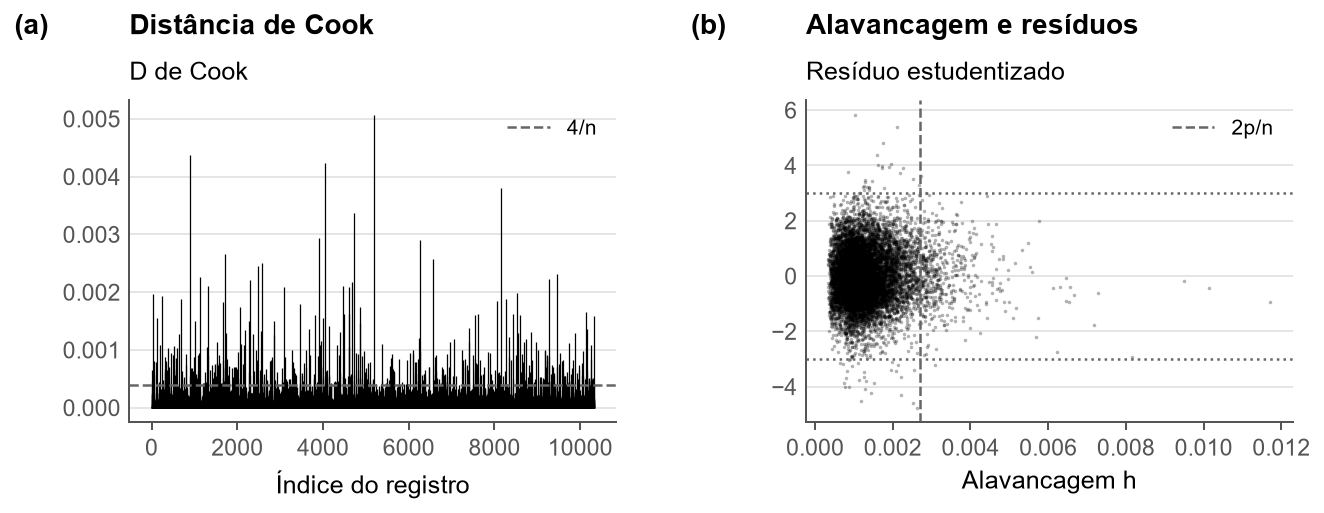
\includegraphics[width=\textwidth]{figuras/influencia.png}
\caption{(a) Distância de Cook por registro, com a referência $4/n$; (b) alavancagem versus resíduo estudentizado, com as referências $2p/n$ e $\pm3$.}
\label{fig:influencia}
\end{figure}

\paragraph{Erros padrão robustos.} Diante da heterocedasticidade detectada, os erros padrão foram recalculados com o estimador HC3, que não pressupõe variância constante. As razões entre os erros robustos e os clássicos variam de 0,90 a 1,10 (Tabela~\ref{tab:vif}), e todos os coeficientes continuam significativos. O de Animais, o menor efeito, tem $p=0{,}0035$. Portanto, \textbf{as conclusões sobre os coeficientes são robustas à violação de E}. O mesmo não vale automaticamente para os intervalos de predição individuais, cuja largura deveria variar com o valor previsto.

\subsection{Comparação com a escala original e desempenho fora da amostra}
\label{sec:comparacao}

O Bloco~\ref{bl:validacao} ajusta, como referência, um modelo com as mesmas 11 candidatas sem nenhuma transformação e compara os dois modelos por validação cruzada em dez partes. Em cada rodada, os modelos são ajustados em 90\% dos registros e avaliados nos 10\% restantes. As previsões do modelo final foram retransformadas para reais com a correção de \textit{smearing} de Duan \cite{duan}, que estima a média condicional, e não a mediana.

\lstinputlisting[caption={Modelo sem transformações e validação cruzada.},label={bl:validacao}]{codigo/b11_validacao.py}

\begin{figure}[H]
\centering
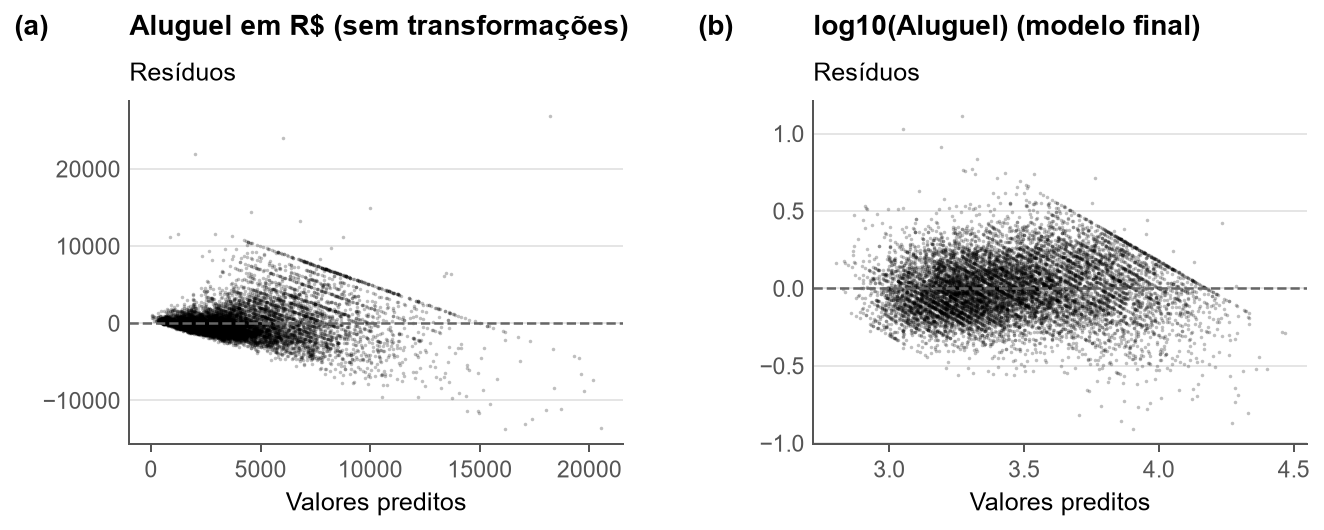
\includegraphics[width=\textwidth]{figuras/comparacao_escalas.png}
\caption{Resíduos versus valores preditos: (a) modelo com aluguel e preditoras em reais, sem transformações; (b) modelo final.}
\label{fig:comparacao}
\end{figure}

O modelo sem transformações tem \Rtwo$=0{,}5902$ (\Rtwoadj$=0{,}5897$), valor que se refere à variabilidade do aluguel em reais e não pode ser comparado diretamente com o 0,6914 do modelo final. Seus resíduos, contudo, mostram problemas graves (Figura~\ref{fig:comparacao}a): a variância cresce fortemente com o valor previsto (funil), a assimetria é de 1,345 e a curtose de 12,280. N e E são claramente violadas, e os intervalos e testes desse modelo não seriam confiáveis. A borda diagonal formada pelos aluguéis de R\$ 15.000 também é visível. As transformações reduziram drasticamente esses problemas (Figura~\ref{fig:comparacao}b).

\begin{table}[H]
\centering
\caption{Desempenho preditivo por validação cruzada em dez partes (previsões sempre fora da amostra de ajuste).}
\label{tab:validacao}
\small
\begin{tabular}{lrr}
\toprule
Métrica (validação cruzada, 10 partes) & Modelo final & Sem transformações \\
\midrule
\Rtwo{} fora da amostra, escala $\log_{10}$ & 0,6906 & \NA \\
RMSE, escala $\log_{10}$ & 0,1907 & \NA \\
\Rtwo{} fora da amostra, em R\$ & 0,5112 & 0,5868 \\
RMSE (R\$) & 2.399 & 2.206 \\
Erro absoluto médio (R\$) & 1.458 & 1.412 \\
Erro percentual absoluto mediano (\%) & 31,3 & 31,3 \\
Previsões não positivas & 0 & 0 \\
\bottomrule
\end{tabular}

\end{table}

Na escala logarítmica, o \Rtwo{} fora da amostra (0,6906) é praticamente igual ao do ajuste (0,6914), e o RMSE (0,1907) coincide com $S$; não há sobreajuste, como esperado quando $n$ é muito maior que o número de parâmetros (Tabela~\ref{tab:validacao}). \textbf{Em reais, porém, o modelo sem transformações tem RMSE menor} (R\$ 2.206 contra R\$ 2.399), e os dois modelos têm erro absoluto médio semelhante e o mesmo erro percentual absoluto mediano, de 31,3\%. Esse resultado não contradiz a escolha das transformações. O OLS na escala original minimiza justamente o erro quadrático em reais, métrica dominada pelos imóveis caros, nos quais os erros são maiores. O modelo logarítmico, por sua vez, modela erros relativos, produz resíduos muito mais próximos das premissas e permite inferência sobre os coeficientes, com erros padrão HC3, e interpretação em termos percentuais. Sua retransformação para a média em reais depende de uma correção que supõe variância constante, hipótese violada, e é afetada pelo teto de R\$ 15.000 no extremo superior.

Em termos práticos, ambos os modelos erram tipicamente cerca de 31\% do aluguel em uma previsão individual. O fator limitante não parece ser a forma funcional, mas a ausência de informações sobre a localização do imóvel dentro da cidade, como bairro ou coordenadas, que é reconhecidamente um dos principais determinantes do aluguel.

\subsection{Síntese: qualidades, limitações e premissas LINE}

\paragraph{Qualidade do ajuste.} O modelo explica 69\% da variabilidade de $\log_{10}(\text{Aluguel})$, com o mesmo desempenho fora da amostra, e seus coeficientes têm sinais e magnitudes plausíveis. Ele fornece um bom ajuste para descrever \textbf{relações médias}, como as diferenças entre cidades e os efeitos de área, mobília e banheiros. Para prever o aluguel de um imóvel específico, porém, o erro típico de cerca de 31\% limita seu uso como ferramenta de avaliação individual.

\begin{table}[H]
\centering
\caption{Síntese de LINE no modelo final. ``Compatível'' significa ausência de evidência forte de violação, e não comprovação da condição.}
\label{tab:line}
\footnotesize
\begin{tabular}{>{\raggedright\arraybackslash}p{2.5cm}
                >{\raggedright\arraybackslash}p{6.0cm}
                >{\raggedright\arraybackslash}p{5.0cm}}
\toprule
Premissa & Evidência & Avaliação \\
\midrule
L: função média linear & LOWESS próximas de zero na região central dos preditos e de cada preditora; média dos resíduos de $-0{,}066$ no decil superior, associado ao teto de R\$ 15.000; desvios em imóveis muito pequenos ou muito grandes & Compatível na maior parte dos dados; violação localizada no extremo superior \\
\addlinespace
I: independência & Dados transversais; duplicatas exatas removidas; localização dentro da cidade ausente; possíveis anúncios do mesmo edifício ou bairro & Não verificável; risco de dependência espacial \\
\addlinespace
N: normalidade & Histograma e Q--Q próximos da normal no centro; assimetria de 0,121 e curtose de 3,755; cinco testes rejeitam com $n=10.320$ & Violação leve, concentrada nas caudas \\
\addlinespace
E: variância constante & Desvio padrão dos resíduos de 0,164 a 0,215 entre decis; Breusch--Pagan, Goldfeld--Quandt e Brown--Forsythe rejeitam & Não sustentada; heterocedasticidade moderada, contornada com EP HC3 \\
\bottomrule
\end{tabular}
\end{table}

A Tabela~\ref{tab:line} resume as premissas, avaliadas conforme as Lições 4 e 7 do STAT 501 \cite{stat501}. Em comparação com o modelo sem transformações, o modelo final representa uma melhora substancial em N e E e permite interpretar os efeitos em termos percentuais. As violações remanescentes têm consequências delimitadas: a heterocedasticidade não altera as conclusões sobre os coeficientes quando se usam erros padrão HC3; o desvio de normalidade é leve; e o desvio de linearidade concentra-se no extremo superior, onde a própria coleta parece limitar o aluguel observado. A independência, por sua vez, não pode ser confirmada com as informações disponíveis.

% =====================================================================
\section{Conclusões}

\begin{itemize}
  \item \textbf{Pré-processamento:} a análise utilizou 10.320 anúncios, após a remoção de 358 duplicatas e de 14 registros implausíveis. Seguro e total foram excluídos por conterem o próprio aluguel, e foi criada a variável \textit{tipo}. Aluguel e área foram transformados com $\log_{10}$, e condomínio e IPTU, com Box-Cox.
  \item \textbf{Seleção:} o \textit{stepwise} com $\alpha_E=\alpha_R=0{,}15$ manteve dez das 11 candidatas e excluiu apenas quartos, redundante diante da área e do número de banheiros. Os critérios AIC e BIC concordaram com essa escolha. Área, cidade e mobília concentram a maior parte do poder explicativo.
  \item \textbf{Efeitos:} com as demais características constantes, o aluguel mediano é de 8\% a 37\% menor nas outras cidades do que em São Paulo; aumenta 4,3\% para cada 10\% de área, 38,8\% quando o imóvel é mobiliado, 9,2\% por banheiro, 4,0\% por vaga e 1,4\% por andar.
  \item \textbf{Ajuste e premissas:} \Rtwo$=0{,}6914$ na escala logarítmica, confirmado por validação cruzada, e teste $F$ altamente significativo. N é aproximadamente atendida; E é violada de forma moderada, com conclusões preservadas pelos erros padrão HC3; L tem desvio no extremo superior, associado ao teto aparente de R\$ 15.000; I não é verificável.
  \item \textbf{Limitações e extensões:} o erro típico de cerca de 31\% em previsões individuais indica que falta informação relevante, principalmente a localização dentro da cidade. Possíveis extensões incluem obter bairro ou coordenadas, modelar o teto explicitamente com regressão censurada (Tobit), investigar interações, como cidade $\times$ área para valores por metro quadrado diferentes entre cidades, e modelar a variância por mínimos quadrados ponderados.
\end{itemize}

As ferramentas de inteligência artificial foram utilizadas como apoio à implementação do código, à análise estatística e à redação do relatório \cite{claude}; esse apoio não substitui a responsabilidade dos autores pela revisão, pela análise e pela interpretação.

\begin{thebibliography}{99}
\bibitem{kaggle}
RUBENSSJR. \textit{Brazilian houses to rent}. Kaggle, 2020. Disponível em: \url{https://www.kaggle.com/datasets/rubenssjr/brasilian-houses-to-rent}. Acesso em: 31 out. 2026.

\bibitem{openml}
OpenML. \textit{Brazilian\_houses} (ID 42688, versão 4). Disponível em: \url{https://www.openml.org/d/42688}. Acesso em: 31 out. 2026.

\bibitem{stat501-10}
Pennsylvania State University. \textit{STAT 501: Regression Methods -- Lesson 10.2, Stepwise Regression}. Disponível em: \url{https://online.stat.psu.edu/stat501/lesson/10/10.2}. Acesso em: 31 out. 2026.

\bibitem{stat501}
Pennsylvania State University. \textit{STAT 501: Regression Methods -- Lessons 4 e 7, Model Assumptions}. Disponível em: \url{https://online.stat.psu.edu/stat501/}. Acesso em: 31 out. 2026.

\bibitem{boxcox}
BOX, G. E. P.; COX, D. R. An analysis of transformations. \textit{Journal of the Royal Statistical Society: Series B}, v. 26, n. 2, p. 211--252, 1964.

\bibitem{duan}
DUAN, N. Smearing estimate: a nonparametric retransformation method. \textit{Journal of the American Statistical Association}, v. 78, n. 383, p. 605--610, 1983.

\bibitem{white}
WHITE, H. A heteroskedasticity-consistent covariance matrix estimator and a direct test for heteroskedasticity. \textit{Econometrica}, v. 48, n. 4, p. 817--838, 1980.

\bibitem{mackinnon}
MACKINNON, J. G.; WHITE, H. Some heteroskedasticity-consistent covariance matrix estimators with improved finite sample properties. \textit{Journal of Econometrics}, v. 29, n. 3, p. 305--325, 1985.

\bibitem{statsmodels}
SEABOLD, S.; PERKTOLD, J. Statsmodels: econometric and statistical modeling with Python. In: \textit{Proceedings of the 9th Python in Science Conference}, 2010.

\bibitem{claude}
Anthropic. \textit{Claude Code}. Assistente de inteligência artificial utilizado como apoio à implementação do código, à análise e à redação do relatório. Disponível em: \url{https://claude.com/claude-code}. Acesso em: 31 out. 2026.
\end{thebibliography}

% =====================================================================
\appendix
\section{Funções auxiliares e execução dos blocos}
\label{ap:auxiliar}

O script \texttt{executar.py} executa os Blocos~\ref{bl:leitura} a \ref{bl:validacao} em sequência, no mesmo ambiente, e grava a saída de cada bloco na pasta \texttt{saidas}. Ao final, executa \texttt{exportar\_tabelas.py}, que apenas converte os resultados já calculados em tabelas \LaTeX{} com formatação numérica brasileira e, por isso, não é reproduzido aqui. O módulo \texttt{graficos.py} contém as funções de visualização, que seguem o mesmo padrão gráfico em tons de cinza da Atividade 1. Para reproduzir a análise, basta executar \texttt{python codigo/executar.py} na pasta do projeto, com o arquivo \texttt{dados/Brazilian\_houses.arff} obtido no OpenML.

\lstinputlisting[title={\texttt{codigo/executar.py}},basicstyle=\ttfamily\scriptsize]{codigo/executar.py}

\lstinputlisting[title={\texttt{codigo/graficos.py}},basicstyle=\ttfamily\scriptsize]{codigo/graficos.py}

\end{document}
